\documentclass{article}
\usepackage[final]{neurips_2025}  % NEURIPS style
\usepackage[hidelinks]{hyperref}  % REQUIRED: clickable links
\usepackage{booktabs}  % REQUIRED: professional tables
\usepackage{graphicx}
\usepackage{amsmath,amssymb}
\usepackage[T1]{fontenc}
\usepackage[utf8]{inputenc}
\usepackage{xspace}
\usepackage{enumitem}
\usepackage[noend]{algpseudocode}

% Import command files
%%%%% MATH NOTATION MACROS %%%%%
% Standard math notation for academic papers
% Import with: %%%%% MATH NOTATION MACROS %%%%%
% Standard math notation for academic papers
% Import with: %%%%% MATH NOTATION MACROS %%%%%
% Standard math notation for academic papers
% Import with: \input{commands/math}

\usepackage{amsmath,amsfonts,bm}

%%%%%%%%%%%%%%%%%%%%%%%%%%%%%%%%%%%%%%%%%%%%%%%%%%%%%%%%%%%%%%%%%
% FIGURE AND SECTION REFERENCES
%%%%%%%%%%%%%%%%%%%%%%%%%%%%%%%%%%%%%%%%%%%%%%%%%%%%%%%%%%%%%%%%%

% Mark sections of captions for referring to divisions of figures
\newcommand{\figleft}{{\em (Left)}}
\newcommand{\figcenter}{{\em (Center)}}
\newcommand{\figright}{{\em (Right)}}
\newcommand{\figtop}{{\em (Top)}}
\newcommand{\figbottom}{{\em (Bottom)}}
\newcommand{\captiona}{{\em (a)}}
\newcommand{\captionb}{{\em (b)}}
\newcommand{\captionc}{{\em (c)}}
\newcommand{\captiond}{{\em (d)}}

% Figure references
\def\figref#1{figure~\ref{#1}}
\def\Figref#1{Figure~\ref{#1}}
\def\twofigref#1#2{figures \ref{#1} and \ref{#2}}
\def\quadfigref#1#2#3#4{figures \ref{#1}, \ref{#2}, \ref{#3} and \ref{#4}}

% Section references
\def\secref#1{section~\ref{#1}}
\def\Secref#1{Section~\ref{#1}}
\def\twosecrefs#1#2{sections \ref{#1} and \ref{#2}}
\def\secrefs#1#2#3{sections \ref{#1}, \ref{#2} and \ref{#3}}

% Equation references
\def\eqref#1{equation~\ref{#1}}
\def\Eqref#1{Equation~\ref{#1}}
\def\plaineqref#1{\ref{#1}}

% Algorithm references
\def\algref#1{algorithm~\ref{#1}}
\def\Algref#1{Algorithm~\ref{#1}}
\def\twoalgref#1#2{algorithms \ref{#1} and \ref{#2}}
\def\Twoalgref#1#2{Algorithms \ref{#1} and \ref{#2}}

% Table references
\def\tabref#1{table~\ref{#1}}
\def\Tabref#1{Table~\ref{#1}}

% Chapter references
\def\chapref#1{chapter~\ref{#1}}
\def\Chapref#1{Chapter~\ref{#1}}

%%%%%%%%%%%%%%%%%%%%%%%%%%%%%%%%%%%%%%%%%%%%%%%%%%%%%%%%%%%%%%%%%
% BASIC MATH DEFINITIONS
%%%%%%%%%%%%%%%%%%%%%%%%%%%%%%%%%%%%%%%%%%%%%%%%%%%%%%%%%%%%%%%%%

\def\ceil#1{\lceil #1 \rceil}
\def\floor#1{\lfloor #1 \rfloor}
\def\1{\bm{1}}
\def\eps{{\epsilon}}

% Common operators
\DeclareMathOperator*{\argmax}{arg\,max}
\DeclareMathOperator*{\argmin}{arg\,min}
\DeclareMathOperator{\sign}{sign}
\DeclareMathOperator{\Tr}{Tr}
\let\ab\allowbreak

%%%%%%%%%%%%%%%%%%%%%%%%%%%%%%%%%%%%%%%%%%%%%%%%%%%%%%%%%%%%%%%%%
% VECTORS (lowercase bold)
%%%%%%%%%%%%%%%%%%%%%%%%%%%%%%%%%%%%%%%%%%%%%%%%%%%%%%%%%%%%%%%%%

\def\vzero{{\bm{0}}}
\def\vone{{\bm{1}}}
\def\vmu{{\bm{\mu}}}
\def\vtheta{{\bm{\theta}}}
\def\va{{\bm{a}}}
\def\vb{{\bm{b}}}
\def\vc{{\bm{c}}}
\def\vd{{\bm{d}}}
\def\ve{{\bm{e}}}
\def\vf{{\bm{f}}}
\def\vg{{\bm{g}}}
\def\vh{{\bm{h}}}
\def\vi{{\bm{i}}}
\def\vj{{\bm{j}}}
\def\vk{{\bm{k}}}
\def\vl{{\bm{l}}}
\def\vm{{\bm{m}}}
\def\vn{{\bm{n}}}
\def\vo{{\bm{o}}}
\def\vp{{\bm{p}}}
\def\vq{{\bm{q}}}
\def\vr{{\bm{r}}}
\def\vs{{\bm{s}}}
\def\vt{{\bm{t}}}
\def\vu{{\bm{u}}}
\def\vv{{\bm{v}}}
\def\vw{{\bm{w}}}
\def\vx{{\bm{x}}}
\def\vy{{\bm{y}}}
\def\vz{{\bm{z}}}

%%%%%%%%%%%%%%%%%%%%%%%%%%%%%%%%%%%%%%%%%%%%%%%%%%%%%%%%%%%%%%%%%
% MATRICES (uppercase bold)
%%%%%%%%%%%%%%%%%%%%%%%%%%%%%%%%%%%%%%%%%%%%%%%%%%%%%%%%%%%%%%%%%

\def\mA{{\bm{A}}}
\def\mB{{\bm{B}}}
\def\mC{{\bm{C}}}
\def\mD{{\bm{D}}}
\def\mE{{\bm{E}}}
\def\mF{{\bm{F}}}
\def\mG{{\bm{G}}}
\def\mH{{\bm{H}}}
\def\mI{{\bm{I}}}
\def\mJ{{\bm{J}}}
\def\mK{{\bm{K}}}
\def\mL{{\bm{L}}}
\def\mM{{\bm{M}}}
\def\mN{{\bm{N}}}
\def\mO{{\bm{O}}}
\def\mP{{\bm{P}}}
\def\mQ{{\bm{Q}}}
\def\mR{{\bm{R}}}
\def\mS{{\bm{S}}}
\def\mT{{\bm{T}}}
\def\mU{{\bm{U}}}
\def\mV{{\bm{V}}}
\def\mW{{\bm{W}}}
\def\mX{{\bm{X}}}
\def\mY{{\bm{Y}}}
\def\mZ{{\bm{Z}}}
\def\mBeta{{\bm{\beta}}}
\def\mPhi{{\bm{\Phi}}}
\def\mLambda{{\bm{\Lambda}}}
\def\mSigma{{\bm{\Sigma}}}

%%%%%%%%%%%%%%%%%%%%%%%%%%%%%%%%%%%%%%%%%%%%%%%%%%%%%%%%%%%%%%%%%
% CALLIGRAPHIC (mathcal)
%%%%%%%%%%%%%%%%%%%%%%%%%%%%%%%%%%%%%%%%%%%%%%%%%%%%%%%%%%%%%%%%%

\def\gA{{\mathcal{A}}}
\def\gB{{\mathcal{B}}}
\def\gC{{\mathcal{C}}}
\def\gD{{\mathcal{D}}}
\def\gE{{\mathcal{E}}}
\def\gF{{\mathcal{F}}}
\def\gG{{\mathcal{G}}}
\def\gH{{\mathcal{H}}}
\def\gI{{\mathcal{I}}}
\def\gJ{{\mathcal{J}}}
\def\gK{{\mathcal{K}}}
\def\gL{{\mathcal{L}}}
\def\gM{{\mathcal{M}}}
\def\gN{{\mathcal{N}}}
\def\gO{{\mathcal{O}}}
\def\gP{{\mathcal{P}}}
\def\gQ{{\mathcal{Q}}}
\def\gR{{\mathcal{R}}}
\def\gS{{\mathcal{S}}}
\def\gT{{\mathcal{T}}}
\def\gU{{\mathcal{U}}}
\def\gV{{\mathcal{V}}}
\def\gW{{\mathcal{W}}}
\def\gX{{\mathcal{X}}}
\def\gY{{\mathcal{Y}}}
\def\gZ{{\mathcal{Z}}}

%%%%%%%%%%%%%%%%%%%%%%%%%%%%%%%%%%%%%%%%%%%%%%%%%%%%%%%%%%%%%%%%%
% SETS (blackboard bold)
%%%%%%%%%%%%%%%%%%%%%%%%%%%%%%%%%%%%%%%%%%%%%%%%%%%%%%%%%%%%%%%%%

\def\sA{{\mathbb{A}}}
\def\sB{{\mathbb{B}}}
\def\sC{{\mathbb{C}}}
\def\sD{{\mathbb{D}}}
\def\sF{{\mathbb{F}}}
\def\sG{{\mathbb{G}}}
\def\sH{{\mathbb{H}}}
\def\sI{{\mathbb{I}}}
\def\sJ{{\mathbb{J}}}
\def\sK{{\mathbb{K}}}
\def\sL{{\mathbb{L}}}
\def\sM{{\mathbb{M}}}
\def\sN{{\mathbb{N}}}
\def\sO{{\mathbb{O}}}
\def\sP{{\mathbb{P}}}
\def\sQ{{\mathbb{Q}}}
\def\sR{{\mathbb{R}}}
\def\sS{{\mathbb{S}}}
\def\sT{{\mathbb{T}}}
\def\sU{{\mathbb{U}}}
\def\sV{{\mathbb{V}}}
\def\sW{{\mathbb{W}}}
\def\sX{{\mathbb{X}}}
\def\sY{{\mathbb{Y}}}
\def\sZ{{\mathbb{Z}}}

%%%%%%%%%%%%%%%%%%%%%%%%%%%%%%%%%%%%%%%%%%%%%%%%%%%%%%%%%%%%%%%%%
% COMMON MATH SHORTCUTS
%%%%%%%%%%%%%%%%%%%%%%%%%%%%%%%%%%%%%%%%%%%%%%%%%%%%%%%%%%%%%%%%%

% Expectation and variance
\newcommand{\E}{\mathbb{E}}
\newcommand{\Var}{\mathrm{Var}}
\newcommand{\Cov}{\mathrm{Cov}}
\newcommand{\R}{\mathbb{R}}

% Datasets
\newcommand{\train}{\mathcal{D}}
\newcommand{\valid}{\mathcal{D_{\mathrm{valid}}}}
\newcommand{\test}{\mathcal{D_{\mathrm{test}}}}

% Distributions
\newcommand{\laplace}{\mathrm{Laplace}}
\newcommand{\Uniform}{\mathrm{Unif}}
\newcommand{\Normal}{\mathrm{Normal}}
\newcommand{\Categorical}{\mathrm{Categorical}}

% Common functions
\newcommand{\softmax}{\mathrm{softmax}}
\newcommand{\sigmoid}{\sigma}
\newcommand{\KL}{D_{\mathrm{KL}}}

% Norms
\newcommand{\normlzero}{L^0}
\newcommand{\normlone}{L^1}
\newcommand{\normltwo}{L^2}
\newcommand{\normlp}{L^p}
\newcommand{\normmax}{L^\infty}

%%%%%%%%%%%%%%%%%%%%%%%%%%%%%%%%%%%%%%%%%%%%%%%%%%%%%%%%%%%%%%%%%
% DEFINITIONS AND HIGHLIGHTING
%%%%%%%%%%%%%%%%%%%%%%%%%%%%%%%%%%%%%%%%%%%%%%%%%%%%%%%%%%%%%%%%%

% Highlight a newly defined term
\newcommand{\newterm}[1]{{\bf #1}}
\newcommand{\defn}[1]{\textbf{#1}}
\newcommand{\defeq}{\mathrel{\stackrel{\textnormal{\tiny def}}{=}}}


\usepackage{amsmath,amsfonts,bm}

%%%%%%%%%%%%%%%%%%%%%%%%%%%%%%%%%%%%%%%%%%%%%%%%%%%%%%%%%%%%%%%%%
% FIGURE AND SECTION REFERENCES
%%%%%%%%%%%%%%%%%%%%%%%%%%%%%%%%%%%%%%%%%%%%%%%%%%%%%%%%%%%%%%%%%

% Mark sections of captions for referring to divisions of figures
\newcommand{\figleft}{{\em (Left)}}
\newcommand{\figcenter}{{\em (Center)}}
\newcommand{\figright}{{\em (Right)}}
\newcommand{\figtop}{{\em (Top)}}
\newcommand{\figbottom}{{\em (Bottom)}}
\newcommand{\captiona}{{\em (a)}}
\newcommand{\captionb}{{\em (b)}}
\newcommand{\captionc}{{\em (c)}}
\newcommand{\captiond}{{\em (d)}}

% Figure references
\def\figref#1{figure~\ref{#1}}
\def\Figref#1{Figure~\ref{#1}}
\def\twofigref#1#2{figures \ref{#1} and \ref{#2}}
\def\quadfigref#1#2#3#4{figures \ref{#1}, \ref{#2}, \ref{#3} and \ref{#4}}

% Section references
\def\secref#1{section~\ref{#1}}
\def\Secref#1{Section~\ref{#1}}
\def\twosecrefs#1#2{sections \ref{#1} and \ref{#2}}
\def\secrefs#1#2#3{sections \ref{#1}, \ref{#2} and \ref{#3}}

% Equation references
\def\eqref#1{equation~\ref{#1}}
\def\Eqref#1{Equation~\ref{#1}}
\def\plaineqref#1{\ref{#1}}

% Algorithm references
\def\algref#1{algorithm~\ref{#1}}
\def\Algref#1{Algorithm~\ref{#1}}
\def\twoalgref#1#2{algorithms \ref{#1} and \ref{#2}}
\def\Twoalgref#1#2{Algorithms \ref{#1} and \ref{#2}}

% Table references
\def\tabref#1{table~\ref{#1}}
\def\Tabref#1{Table~\ref{#1}}

% Chapter references
\def\chapref#1{chapter~\ref{#1}}
\def\Chapref#1{Chapter~\ref{#1}}

%%%%%%%%%%%%%%%%%%%%%%%%%%%%%%%%%%%%%%%%%%%%%%%%%%%%%%%%%%%%%%%%%
% BASIC MATH DEFINITIONS
%%%%%%%%%%%%%%%%%%%%%%%%%%%%%%%%%%%%%%%%%%%%%%%%%%%%%%%%%%%%%%%%%

\def\ceil#1{\lceil #1 \rceil}
\def\floor#1{\lfloor #1 \rfloor}
\def\1{\bm{1}}
\def\eps{{\epsilon}}

% Common operators
\DeclareMathOperator*{\argmax}{arg\,max}
\DeclareMathOperator*{\argmin}{arg\,min}
\DeclareMathOperator{\sign}{sign}
\DeclareMathOperator{\Tr}{Tr}
\let\ab\allowbreak

%%%%%%%%%%%%%%%%%%%%%%%%%%%%%%%%%%%%%%%%%%%%%%%%%%%%%%%%%%%%%%%%%
% VECTORS (lowercase bold)
%%%%%%%%%%%%%%%%%%%%%%%%%%%%%%%%%%%%%%%%%%%%%%%%%%%%%%%%%%%%%%%%%

\def\vzero{{\bm{0}}}
\def\vone{{\bm{1}}}
\def\vmu{{\bm{\mu}}}
\def\vtheta{{\bm{\theta}}}
\def\va{{\bm{a}}}
\def\vb{{\bm{b}}}
\def\vc{{\bm{c}}}
\def\vd{{\bm{d}}}
\def\ve{{\bm{e}}}
\def\vf{{\bm{f}}}
\def\vg{{\bm{g}}}
\def\vh{{\bm{h}}}
\def\vi{{\bm{i}}}
\def\vj{{\bm{j}}}
\def\vk{{\bm{k}}}
\def\vl{{\bm{l}}}
\def\vm{{\bm{m}}}
\def\vn{{\bm{n}}}
\def\vo{{\bm{o}}}
\def\vp{{\bm{p}}}
\def\vq{{\bm{q}}}
\def\vr{{\bm{r}}}
\def\vs{{\bm{s}}}
\def\vt{{\bm{t}}}
\def\vu{{\bm{u}}}
\def\vv{{\bm{v}}}
\def\vw{{\bm{w}}}
\def\vx{{\bm{x}}}
\def\vy{{\bm{y}}}
\def\vz{{\bm{z}}}

%%%%%%%%%%%%%%%%%%%%%%%%%%%%%%%%%%%%%%%%%%%%%%%%%%%%%%%%%%%%%%%%%
% MATRICES (uppercase bold)
%%%%%%%%%%%%%%%%%%%%%%%%%%%%%%%%%%%%%%%%%%%%%%%%%%%%%%%%%%%%%%%%%

\def\mA{{\bm{A}}}
\def\mB{{\bm{B}}}
\def\mC{{\bm{C}}}
\def\mD{{\bm{D}}}
\def\mE{{\bm{E}}}
\def\mF{{\bm{F}}}
\def\mG{{\bm{G}}}
\def\mH{{\bm{H}}}
\def\mI{{\bm{I}}}
\def\mJ{{\bm{J}}}
\def\mK{{\bm{K}}}
\def\mL{{\bm{L}}}
\def\mM{{\bm{M}}}
\def\mN{{\bm{N}}}
\def\mO{{\bm{O}}}
\def\mP{{\bm{P}}}
\def\mQ{{\bm{Q}}}
\def\mR{{\bm{R}}}
\def\mS{{\bm{S}}}
\def\mT{{\bm{T}}}
\def\mU{{\bm{U}}}
\def\mV{{\bm{V}}}
\def\mW{{\bm{W}}}
\def\mX{{\bm{X}}}
\def\mY{{\bm{Y}}}
\def\mZ{{\bm{Z}}}
\def\mBeta{{\bm{\beta}}}
\def\mPhi{{\bm{\Phi}}}
\def\mLambda{{\bm{\Lambda}}}
\def\mSigma{{\bm{\Sigma}}}

%%%%%%%%%%%%%%%%%%%%%%%%%%%%%%%%%%%%%%%%%%%%%%%%%%%%%%%%%%%%%%%%%
% CALLIGRAPHIC (mathcal)
%%%%%%%%%%%%%%%%%%%%%%%%%%%%%%%%%%%%%%%%%%%%%%%%%%%%%%%%%%%%%%%%%

\def\gA{{\mathcal{A}}}
\def\gB{{\mathcal{B}}}
\def\gC{{\mathcal{C}}}
\def\gD{{\mathcal{D}}}
\def\gE{{\mathcal{E}}}
\def\gF{{\mathcal{F}}}
\def\gG{{\mathcal{G}}}
\def\gH{{\mathcal{H}}}
\def\gI{{\mathcal{I}}}
\def\gJ{{\mathcal{J}}}
\def\gK{{\mathcal{K}}}
\def\gL{{\mathcal{L}}}
\def\gM{{\mathcal{M}}}
\def\gN{{\mathcal{N}}}
\def\gO{{\mathcal{O}}}
\def\gP{{\mathcal{P}}}
\def\gQ{{\mathcal{Q}}}
\def\gR{{\mathcal{R}}}
\def\gS{{\mathcal{S}}}
\def\gT{{\mathcal{T}}}
\def\gU{{\mathcal{U}}}
\def\gV{{\mathcal{V}}}
\def\gW{{\mathcal{W}}}
\def\gX{{\mathcal{X}}}
\def\gY{{\mathcal{Y}}}
\def\gZ{{\mathcal{Z}}}

%%%%%%%%%%%%%%%%%%%%%%%%%%%%%%%%%%%%%%%%%%%%%%%%%%%%%%%%%%%%%%%%%
% SETS (blackboard bold)
%%%%%%%%%%%%%%%%%%%%%%%%%%%%%%%%%%%%%%%%%%%%%%%%%%%%%%%%%%%%%%%%%

\def\sA{{\mathbb{A}}}
\def\sB{{\mathbb{B}}}
\def\sC{{\mathbb{C}}}
\def\sD{{\mathbb{D}}}
\def\sF{{\mathbb{F}}}
\def\sG{{\mathbb{G}}}
\def\sH{{\mathbb{H}}}
\def\sI{{\mathbb{I}}}
\def\sJ{{\mathbb{J}}}
\def\sK{{\mathbb{K}}}
\def\sL{{\mathbb{L}}}
\def\sM{{\mathbb{M}}}
\def\sN{{\mathbb{N}}}
\def\sO{{\mathbb{O}}}
\def\sP{{\mathbb{P}}}
\def\sQ{{\mathbb{Q}}}
\def\sR{{\mathbb{R}}}
\def\sS{{\mathbb{S}}}
\def\sT{{\mathbb{T}}}
\def\sU{{\mathbb{U}}}
\def\sV{{\mathbb{V}}}
\def\sW{{\mathbb{W}}}
\def\sX{{\mathbb{X}}}
\def\sY{{\mathbb{Y}}}
\def\sZ{{\mathbb{Z}}}

%%%%%%%%%%%%%%%%%%%%%%%%%%%%%%%%%%%%%%%%%%%%%%%%%%%%%%%%%%%%%%%%%
% COMMON MATH SHORTCUTS
%%%%%%%%%%%%%%%%%%%%%%%%%%%%%%%%%%%%%%%%%%%%%%%%%%%%%%%%%%%%%%%%%

% Expectation and variance
\newcommand{\E}{\mathbb{E}}
\newcommand{\Var}{\mathrm{Var}}
\newcommand{\Cov}{\mathrm{Cov}}
\newcommand{\R}{\mathbb{R}}

% Datasets
\newcommand{\train}{\mathcal{D}}
\newcommand{\valid}{\mathcal{D_{\mathrm{valid}}}}
\newcommand{\test}{\mathcal{D_{\mathrm{test}}}}

% Distributions
\newcommand{\laplace}{\mathrm{Laplace}}
\newcommand{\Uniform}{\mathrm{Unif}}
\newcommand{\Normal}{\mathrm{Normal}}
\newcommand{\Categorical}{\mathrm{Categorical}}

% Common functions
\newcommand{\softmax}{\mathrm{softmax}}
\newcommand{\sigmoid}{\sigma}
\newcommand{\KL}{D_{\mathrm{KL}}}

% Norms
\newcommand{\normlzero}{L^0}
\newcommand{\normlone}{L^1}
\newcommand{\normltwo}{L^2}
\newcommand{\normlp}{L^p}
\newcommand{\normmax}{L^\infty}

%%%%%%%%%%%%%%%%%%%%%%%%%%%%%%%%%%%%%%%%%%%%%%%%%%%%%%%%%%%%%%%%%
% DEFINITIONS AND HIGHLIGHTING
%%%%%%%%%%%%%%%%%%%%%%%%%%%%%%%%%%%%%%%%%%%%%%%%%%%%%%%%%%%%%%%%%

% Highlight a newly defined term
\newcommand{\newterm}[1]{{\bf #1}}
\newcommand{\defn}[1]{\textbf{#1}}
\newcommand{\defeq}{\mathrel{\stackrel{\textnormal{\tiny def}}{=}}}


\usepackage{amsmath,amsfonts,bm}

%%%%%%%%%%%%%%%%%%%%%%%%%%%%%%%%%%%%%%%%%%%%%%%%%%%%%%%%%%%%%%%%%
% FIGURE AND SECTION REFERENCES
%%%%%%%%%%%%%%%%%%%%%%%%%%%%%%%%%%%%%%%%%%%%%%%%%%%%%%%%%%%%%%%%%

% Mark sections of captions for referring to divisions of figures
\newcommand{\figleft}{{\em (Left)}}
\newcommand{\figcenter}{{\em (Center)}}
\newcommand{\figright}{{\em (Right)}}
\newcommand{\figtop}{{\em (Top)}}
\newcommand{\figbottom}{{\em (Bottom)}}
\newcommand{\captiona}{{\em (a)}}
\newcommand{\captionb}{{\em (b)}}
\newcommand{\captionc}{{\em (c)}}
\newcommand{\captiond}{{\em (d)}}

% Figure references
\def\figref#1{figure~\ref{#1}}
\def\Figref#1{Figure~\ref{#1}}
\def\twofigref#1#2{figures \ref{#1} and \ref{#2}}
\def\quadfigref#1#2#3#4{figures \ref{#1}, \ref{#2}, \ref{#3} and \ref{#4}}

% Section references
\def\secref#1{section~\ref{#1}}
\def\Secref#1{Section~\ref{#1}}
\def\twosecrefs#1#2{sections \ref{#1} and \ref{#2}}
\def\secrefs#1#2#3{sections \ref{#1}, \ref{#2} and \ref{#3}}

% Equation references
\def\eqref#1{equation~\ref{#1}}
\def\Eqref#1{Equation~\ref{#1}}
\def\plaineqref#1{\ref{#1}}

% Algorithm references
\def\algref#1{algorithm~\ref{#1}}
\def\Algref#1{Algorithm~\ref{#1}}
\def\twoalgref#1#2{algorithms \ref{#1} and \ref{#2}}
\def\Twoalgref#1#2{Algorithms \ref{#1} and \ref{#2}}

% Table references
\def\tabref#1{table~\ref{#1}}
\def\Tabref#1{Table~\ref{#1}}

% Chapter references
\def\chapref#1{chapter~\ref{#1}}
\def\Chapref#1{Chapter~\ref{#1}}

%%%%%%%%%%%%%%%%%%%%%%%%%%%%%%%%%%%%%%%%%%%%%%%%%%%%%%%%%%%%%%%%%
% BASIC MATH DEFINITIONS
%%%%%%%%%%%%%%%%%%%%%%%%%%%%%%%%%%%%%%%%%%%%%%%%%%%%%%%%%%%%%%%%%

\def\ceil#1{\lceil #1 \rceil}
\def\floor#1{\lfloor #1 \rfloor}
\def\1{\bm{1}}
\def\eps{{\epsilon}}

% Common operators
\DeclareMathOperator*{\argmax}{arg\,max}
\DeclareMathOperator*{\argmin}{arg\,min}
\DeclareMathOperator{\sign}{sign}
\DeclareMathOperator{\Tr}{Tr}
\let\ab\allowbreak

%%%%%%%%%%%%%%%%%%%%%%%%%%%%%%%%%%%%%%%%%%%%%%%%%%%%%%%%%%%%%%%%%
% VECTORS (lowercase bold)
%%%%%%%%%%%%%%%%%%%%%%%%%%%%%%%%%%%%%%%%%%%%%%%%%%%%%%%%%%%%%%%%%

\def\vzero{{\bm{0}}}
\def\vone{{\bm{1}}}
\def\vmu{{\bm{\mu}}}
\def\vtheta{{\bm{\theta}}}
\def\va{{\bm{a}}}
\def\vb{{\bm{b}}}
\def\vc{{\bm{c}}}
\def\vd{{\bm{d}}}
\def\ve{{\bm{e}}}
\def\vf{{\bm{f}}}
\def\vg{{\bm{g}}}
\def\vh{{\bm{h}}}
\def\vi{{\bm{i}}}
\def\vj{{\bm{j}}}
\def\vk{{\bm{k}}}
\def\vl{{\bm{l}}}
\def\vm{{\bm{m}}}
\def\vn{{\bm{n}}}
\def\vo{{\bm{o}}}
\def\vp{{\bm{p}}}
\def\vq{{\bm{q}}}
\def\vr{{\bm{r}}}
\def\vs{{\bm{s}}}
\def\vt{{\bm{t}}}
\def\vu{{\bm{u}}}
\def\vv{{\bm{v}}}
\def\vw{{\bm{w}}}
\def\vx{{\bm{x}}}
\def\vy{{\bm{y}}}
\def\vz{{\bm{z}}}

%%%%%%%%%%%%%%%%%%%%%%%%%%%%%%%%%%%%%%%%%%%%%%%%%%%%%%%%%%%%%%%%%
% MATRICES (uppercase bold)
%%%%%%%%%%%%%%%%%%%%%%%%%%%%%%%%%%%%%%%%%%%%%%%%%%%%%%%%%%%%%%%%%

\def\mA{{\bm{A}}}
\def\mB{{\bm{B}}}
\def\mC{{\bm{C}}}
\def\mD{{\bm{D}}}
\def\mE{{\bm{E}}}
\def\mF{{\bm{F}}}
\def\mG{{\bm{G}}}
\def\mH{{\bm{H}}}
\def\mI{{\bm{I}}}
\def\mJ{{\bm{J}}}
\def\mK{{\bm{K}}}
\def\mL{{\bm{L}}}
\def\mM{{\bm{M}}}
\def\mN{{\bm{N}}}
\def\mO{{\bm{O}}}
\def\mP{{\bm{P}}}
\def\mQ{{\bm{Q}}}
\def\mR{{\bm{R}}}
\def\mS{{\bm{S}}}
\def\mT{{\bm{T}}}
\def\mU{{\bm{U}}}
\def\mV{{\bm{V}}}
\def\mW{{\bm{W}}}
\def\mX{{\bm{X}}}
\def\mY{{\bm{Y}}}
\def\mZ{{\bm{Z}}}
\def\mBeta{{\bm{\beta}}}
\def\mPhi{{\bm{\Phi}}}
\def\mLambda{{\bm{\Lambda}}}
\def\mSigma{{\bm{\Sigma}}}

%%%%%%%%%%%%%%%%%%%%%%%%%%%%%%%%%%%%%%%%%%%%%%%%%%%%%%%%%%%%%%%%%
% CALLIGRAPHIC (mathcal)
%%%%%%%%%%%%%%%%%%%%%%%%%%%%%%%%%%%%%%%%%%%%%%%%%%%%%%%%%%%%%%%%%

\def\gA{{\mathcal{A}}}
\def\gB{{\mathcal{B}}}
\def\gC{{\mathcal{C}}}
\def\gD{{\mathcal{D}}}
\def\gE{{\mathcal{E}}}
\def\gF{{\mathcal{F}}}
\def\gG{{\mathcal{G}}}
\def\gH{{\mathcal{H}}}
\def\gI{{\mathcal{I}}}
\def\gJ{{\mathcal{J}}}
\def\gK{{\mathcal{K}}}
\def\gL{{\mathcal{L}}}
\def\gM{{\mathcal{M}}}
\def\gN{{\mathcal{N}}}
\def\gO{{\mathcal{O}}}
\def\gP{{\mathcal{P}}}
\def\gQ{{\mathcal{Q}}}
\def\gR{{\mathcal{R}}}
\def\gS{{\mathcal{S}}}
\def\gT{{\mathcal{T}}}
\def\gU{{\mathcal{U}}}
\def\gV{{\mathcal{V}}}
\def\gW{{\mathcal{W}}}
\def\gX{{\mathcal{X}}}
\def\gY{{\mathcal{Y}}}
\def\gZ{{\mathcal{Z}}}

%%%%%%%%%%%%%%%%%%%%%%%%%%%%%%%%%%%%%%%%%%%%%%%%%%%%%%%%%%%%%%%%%
% SETS (blackboard bold)
%%%%%%%%%%%%%%%%%%%%%%%%%%%%%%%%%%%%%%%%%%%%%%%%%%%%%%%%%%%%%%%%%

\def\sA{{\mathbb{A}}}
\def\sB{{\mathbb{B}}}
\def\sC{{\mathbb{C}}}
\def\sD{{\mathbb{D}}}
\def\sF{{\mathbb{F}}}
\def\sG{{\mathbb{G}}}
\def\sH{{\mathbb{H}}}
\def\sI{{\mathbb{I}}}
\def\sJ{{\mathbb{J}}}
\def\sK{{\mathbb{K}}}
\def\sL{{\mathbb{L}}}
\def\sM{{\mathbb{M}}}
\def\sN{{\mathbb{N}}}
\def\sO{{\mathbb{O}}}
\def\sP{{\mathbb{P}}}
\def\sQ{{\mathbb{Q}}}
\def\sR{{\mathbb{R}}}
\def\sS{{\mathbb{S}}}
\def\sT{{\mathbb{T}}}
\def\sU{{\mathbb{U}}}
\def\sV{{\mathbb{V}}}
\def\sW{{\mathbb{W}}}
\def\sX{{\mathbb{X}}}
\def\sY{{\mathbb{Y}}}
\def\sZ{{\mathbb{Z}}}

%%%%%%%%%%%%%%%%%%%%%%%%%%%%%%%%%%%%%%%%%%%%%%%%%%%%%%%%%%%%%%%%%
% COMMON MATH SHORTCUTS
%%%%%%%%%%%%%%%%%%%%%%%%%%%%%%%%%%%%%%%%%%%%%%%%%%%%%%%%%%%%%%%%%

% Expectation and variance
\newcommand{\E}{\mathbb{E}}
\newcommand{\Var}{\mathrm{Var}}
\newcommand{\Cov}{\mathrm{Cov}}
\newcommand{\R}{\mathbb{R}}

% Datasets
\newcommand{\train}{\mathcal{D}}
\newcommand{\valid}{\mathcal{D_{\mathrm{valid}}}}
\newcommand{\test}{\mathcal{D_{\mathrm{test}}}}

% Distributions
\newcommand{\laplace}{\mathrm{Laplace}}
\newcommand{\Uniform}{\mathrm{Unif}}
\newcommand{\Normal}{\mathrm{Normal}}
\newcommand{\Categorical}{\mathrm{Categorical}}

% Common functions
\newcommand{\softmax}{\mathrm{softmax}}
\newcommand{\sigmoid}{\sigma}
\newcommand{\KL}{D_{\mathrm{KL}}}

% Norms
\newcommand{\normlzero}{L^0}
\newcommand{\normlone}{L^1}
\newcommand{\normltwo}{L^2}
\newcommand{\normlp}{L^p}
\newcommand{\normmax}{L^\infty}

%%%%%%%%%%%%%%%%%%%%%%%%%%%%%%%%%%%%%%%%%%%%%%%%%%%%%%%%%%%%%%%%%
% DEFINITIONS AND HIGHLIGHTING
%%%%%%%%%%%%%%%%%%%%%%%%%%%%%%%%%%%%%%%%%%%%%%%%%%%%%%%%%%%%%%%%%

% Highlight a newly defined term
\newcommand{\newterm}[1]{{\bf #1}}
\newcommand{\defn}[1]{\textbf{#1}}
\newcommand{\defeq}{\mathrel{\stackrel{\textnormal{\tiny def}}{=}}}

%%%%% GENERAL FORMATTING MACROS %%%%%
% General formatting and styling macros for academic papers
% Import with: %%%%% GENERAL FORMATTING MACROS %%%%%
% General formatting and styling macros for academic papers
% Import with: %%%%% GENERAL FORMATTING MACROS %%%%%
% General formatting and styling macros for academic papers
% Import with: \input{commands/general}

%%%%%%%%%%%%%%%%%%%%%%%%%%%%%%%%%%%%%%%%%%%%%%%%%%%%%%%%%%%%%%%%%
% PARAGRAPH AND TEXT FORMATTING
%%%%%%%%%%%%%%%%%%%%%%%%%%%%%%%%%%%%%%%%%%%%%%%%%%%%%%%%%%%%%%%%%

% Bold paragraph headers (use: \para{Header.} followed by text)
\newcommand{\para}[1]{\noindent \textbf{#1}}

% Cut content for space (content is hidden but preserved in source)
\newcommand{\cutforspace}[1]{}

% Response/rebuttal formatting for reviews
\newcommand{\response}[1]{\vspace{3pt}\hrule\vspace{3pt}\textbf{#1:}}

%%%%%%%%%%%%%%%%%%%%%%%%%%%%%%%%%%%%%%%%%%%%%%%%%%%%%%%%%%%%%%%%%
% RESULT HIGHLIGHTING
%%%%%%%%%%%%%%%%%%%%%%%%%%%%%%%%%%%%%%%%%%%%%%%%%%%%%%%%%%%%%%%%%

\usepackage{xcolor}
\usepackage{bm}

% Colors for result arrows
\definecolor{pastelgreen}{RGB}{50,205,50}

% Arrows for showing improvement/decline in results
\newcommand{\increase}{\textcolor{pastelgreen}{\bm{$\uparrow$}}}
\newcommand{\decrease}{\textcolor{red}{\bm{$\downarrow$}}}

% Phantom star for alignment in tables (use where no significance marker needed)
\newcommand{\pstar}{\phantom{*}}

%%%%%%%%%%%%%%%%%%%%%%%%%%%%%%%%%%%%%%%%%%%%%%%%%%%%%%%%%%%%%%%%%
% HIGHLIGHT BOXES
%%%%%%%%%%%%%%%%%%%%%%%%%%%%%%%%%%%%%%%%%%%%%%%%%%%%%%%%%%%%%%%%%

% Background colors for highlight boxes
\definecolor{aigold}{RGB}{244,210,1}
\definecolor{aigreen}{RGB}{213,245,227}
\definecolor{humanpurple}{RGB}{235,222,240}
\definecolor{aired}{RGB}{255,180,181}
\definecolor{mypurple}{RGB}{147,112,219}
\definecolor{myorange}{RGB}{255,165,0}
\definecolor{commentgray}{RGB}{86,101,115}
\definecolor{mygray}{RGB}{169,169,169}

% Highlight boxes for examples, quotes, etc.
\newcommand{\lightgreen}[1]{\fcolorbox{aigreen}{aigreen}{\parbox{\linewidth}{#1}}}
\newcommand{\lightred}[1]{\colorbox{aired}{\parbox{\linewidth}{#1}}}

%%%%%%%%%%%%%%%%%%%%%%%%%%%%%%%%%%%%%%%%%%%%%%%%%%%%%%%%%%%%%%%%%
% ALGORITHM STYLING
%%%%%%%%%%%%%%%%%%%%%%%%%%%%%%%%%%%%%%%%%%%%%%%%%%%%%%%%%%%%%%%%%

% Comment style for algorithms (triangleright marker)
\newcommand{\rightcomment}[1]{\(\triangleright\) {\small \it #1}}

% Equation comments
\newcommand{\eqcomment}[1]{\addtocounter{equation}{1}\tag*{\rightcomment{#1}\quad(\theequation)}}

% Algorithm formatting (requires algorithm and algpseudocode packages)
% \usepackage{algorithm}
% \usepackage[noend]{algpseudocode}

% Customize algorithm appearance
\renewcommand{\algorithmicindent}{9pt}
% \renewcommand\algorithmicdo{:}
% \renewcommand\algorithmicthen{:}

% Algorithm input/output
% \algnewcommand\algorithmicinput{{\bfseries Input:}}
% \algnewcommand\INPUT{\item[\algorithmicinput]}
% \algnewcommand\algorithmicoutput{{\bfseries Output:}}
% \algnewcommand\OUTPUT{\item[\algorithmicoutput]}

%%%%%%%%%%%%%%%%%%%%%%%%%%%%%%%%%%%%%%%%%%%%%%%%%%%%%%%%%%%%%%%%%
% CODE LISTINGS
%%%%%%%%%%%%%%%%%%%%%%%%%%%%%%%%%%%%%%%%%%%%%%%%%%%%%%%%%%%%%%%%%

\usepackage{listings}

\definecolor{codepurple}{RGB}{128,0,128}

\lstdefinestyle{datalogstyle}{
    basicstyle={\tt \scriptsize},
    xleftmargin={6pt},
    xrightmargin={6pt},
    columns=flexible,
    breakindent=0pt,
    breaklines=true,
    frame=tb,
    stepnumber=1,
    firstnumber=1,
    numberfirstline=true,
    tabsize=2,
    extendedchars=true,
    columns=fullflexible,
    keepspaces=true,
    escapeinside={@}{@},
    captionpos=b,
    commentstyle=\color{black!65},
    numberstyle=\tiny\color{black!65},
    stringstyle=\color{codepurple},
    breakatwhitespace=false,
    mathescape=true,
    numbersep=5pt,
    showspaces=false,
    showstringspaces=false,
    showtabs=false,
    aboveskip={0.8\baselineskip},
    belowskip={0.2\baselineskip},
}
\lstset{style=datalogstyle}

% Rename listings to "Example"
\renewcommand{\lstlistingname}{Example}

% Vertical dots for code continuation
\newcommand{\progvdots}{\\[-4pt]$\vdots$}

%%%%%%%%%%%%%%%%%%%%%%%%%%%%%%%%%%%%%%%%%%%%%%%%%%%%%%%%%%%%%%%%%
% AUTHOR COMMENT SYSTEM
%%%%%%%%%%%%%%%%%%%%%%%%%%%%%%%%%%%%%%%%%%%%%%%%%%%%%%%%%%%%%%%%%

% Toggle to hide/show comments (uncomment \hidecommentstrue to hide)
\newif\ifhidecomments
% \hidecommentstrue

% Define author comments (add your own authors here)
% Each author gets a unique color
\ifhidecomments
    % Hidden mode - comments are invisible
    \newcommand{\authorone}[1]{}
    \newcommand{\authortwo}[1]{}
    \newcommand{\authorthree}[1]{}
\else
    % Visible mode - comments shown in color
    \newcommand{\authorone}[1]{\textcolor{blue}{[\textsc{AuthorOne}: #1]}}
    \newcommand{\authortwo}[1]{\textcolor{green!70!blue}{[\textsc{AuthorTwo}: #1]}}
    \newcommand{\authorthree}[1]{\textcolor{magenta!80!brown}{[\textsc{AuthorThree}: #1]}}
\fi

% Generic fixme/todo command
\newcommand{\fixme}[1]{\textcolor{red}{[FIXME: #1]}}

%%%%%%%%%%%%%%%%%%%%%%%%%%%%%%%%%%%%%%%%%%%%%%%%%%%%%%%%%%%%%%%%%
% SPACING CONFIGURATION
%%%%%%%%%%%%%%%%%%%%%%%%%%%%%%%%%%%%%%%%%%%%%%%%%%%%%%%%%%%%%%%%%

% Tight spacing for figures and tables (adjust as needed)
% \captionsetup[subfigure]{aboveskip=2pt,belowskip=2pt}
% \captionsetup[table]{aboveskip=4pt,belowskip=4pt}
% \captionsetup[figure]{aboveskip=4pt,belowskip=4pt}
% \setlength{\dbltextfloatsep}{11pt}
% \setlength{\dblfloatsep}{11pt}
% \setlength{\floatsep}{11pt}
% \setlength{\textfloatsep}{11pt}

%%%%%%%%%%%%%%%%%%%%%%%%%%%%%%%%%%%%%%%%%%%%%%%%%%%%%%%%%%%%%%%%%
% MISCELLANEOUS
%%%%%%%%%%%%%%%%%%%%%%%%%%%%%%%%%%%%%%%%%%%%%%%%%%%%%%%%%%%%%%%%%

% Ordinals
\renewcommand{\th}{\textsuperscript{th}\xspace}

% Special tokens
\newcommand{\bos}{\textsc{bos}\xspace}
\newcommand{\eos}{\textsc{eos}\xspace}

% Inverse notation
\newcommand{\inv}[1]{#1^{\scriptscriptstyle-\!1}}


%%%%%%%%%%%%%%%%%%%%%%%%%%%%%%%%%%%%%%%%%%%%%%%%%%%%%%%%%%%%%%%%%
% PARAGRAPH AND TEXT FORMATTING
%%%%%%%%%%%%%%%%%%%%%%%%%%%%%%%%%%%%%%%%%%%%%%%%%%%%%%%%%%%%%%%%%

% Bold paragraph headers (use: \para{Header.} followed by text)
\newcommand{\para}[1]{\noindent \textbf{#1}}

% Cut content for space (content is hidden but preserved in source)
\newcommand{\cutforspace}[1]{}

% Response/rebuttal formatting for reviews
\newcommand{\response}[1]{\vspace{3pt}\hrule\vspace{3pt}\textbf{#1:}}

%%%%%%%%%%%%%%%%%%%%%%%%%%%%%%%%%%%%%%%%%%%%%%%%%%%%%%%%%%%%%%%%%
% RESULT HIGHLIGHTING
%%%%%%%%%%%%%%%%%%%%%%%%%%%%%%%%%%%%%%%%%%%%%%%%%%%%%%%%%%%%%%%%%

\usepackage{xcolor}
\usepackage{bm}

% Colors for result arrows
\definecolor{pastelgreen}{RGB}{50,205,50}

% Arrows for showing improvement/decline in results
\newcommand{\increase}{\textcolor{pastelgreen}{\bm{$\uparrow$}}}
\newcommand{\decrease}{\textcolor{red}{\bm{$\downarrow$}}}

% Phantom star for alignment in tables (use where no significance marker needed)
\newcommand{\pstar}{\phantom{*}}

%%%%%%%%%%%%%%%%%%%%%%%%%%%%%%%%%%%%%%%%%%%%%%%%%%%%%%%%%%%%%%%%%
% HIGHLIGHT BOXES
%%%%%%%%%%%%%%%%%%%%%%%%%%%%%%%%%%%%%%%%%%%%%%%%%%%%%%%%%%%%%%%%%

% Background colors for highlight boxes
\definecolor{aigold}{RGB}{244,210,1}
\definecolor{aigreen}{RGB}{213,245,227}
\definecolor{humanpurple}{RGB}{235,222,240}
\definecolor{aired}{RGB}{255,180,181}
\definecolor{mypurple}{RGB}{147,112,219}
\definecolor{myorange}{RGB}{255,165,0}
\definecolor{commentgray}{RGB}{86,101,115}
\definecolor{mygray}{RGB}{169,169,169}

% Highlight boxes for examples, quotes, etc.
\newcommand{\lightgreen}[1]{\fcolorbox{aigreen}{aigreen}{\parbox{\linewidth}{#1}}}
\newcommand{\lightred}[1]{\colorbox{aired}{\parbox{\linewidth}{#1}}}

%%%%%%%%%%%%%%%%%%%%%%%%%%%%%%%%%%%%%%%%%%%%%%%%%%%%%%%%%%%%%%%%%
% ALGORITHM STYLING
%%%%%%%%%%%%%%%%%%%%%%%%%%%%%%%%%%%%%%%%%%%%%%%%%%%%%%%%%%%%%%%%%

% Comment style for algorithms (triangleright marker)
\newcommand{\rightcomment}[1]{\(\triangleright\) {\small \it #1}}

% Equation comments
\newcommand{\eqcomment}[1]{\addtocounter{equation}{1}\tag*{\rightcomment{#1}\quad(\theequation)}}

% Algorithm formatting (requires algorithm and algpseudocode packages)
% \usepackage{algorithm}
% \usepackage[noend]{algpseudocode}

% Customize algorithm appearance
\renewcommand{\algorithmicindent}{9pt}
% \renewcommand\algorithmicdo{:}
% \renewcommand\algorithmicthen{:}

% Algorithm input/output
% \algnewcommand\algorithmicinput{{\bfseries Input:}}
% \algnewcommand\INPUT{\item[\algorithmicinput]}
% \algnewcommand\algorithmicoutput{{\bfseries Output:}}
% \algnewcommand\OUTPUT{\item[\algorithmicoutput]}

%%%%%%%%%%%%%%%%%%%%%%%%%%%%%%%%%%%%%%%%%%%%%%%%%%%%%%%%%%%%%%%%%
% CODE LISTINGS
%%%%%%%%%%%%%%%%%%%%%%%%%%%%%%%%%%%%%%%%%%%%%%%%%%%%%%%%%%%%%%%%%

\usepackage{listings}

\definecolor{codepurple}{RGB}{128,0,128}

\lstdefinestyle{datalogstyle}{
    basicstyle={\tt \scriptsize},
    xleftmargin={6pt},
    xrightmargin={6pt},
    columns=flexible,
    breakindent=0pt,
    breaklines=true,
    frame=tb,
    stepnumber=1,
    firstnumber=1,
    numberfirstline=true,
    tabsize=2,
    extendedchars=true,
    columns=fullflexible,
    keepspaces=true,
    escapeinside={@}{@},
    captionpos=b,
    commentstyle=\color{black!65},
    numberstyle=\tiny\color{black!65},
    stringstyle=\color{codepurple},
    breakatwhitespace=false,
    mathescape=true,
    numbersep=5pt,
    showspaces=false,
    showstringspaces=false,
    showtabs=false,
    aboveskip={0.8\baselineskip},
    belowskip={0.2\baselineskip},
}
\lstset{style=datalogstyle}

% Rename listings to "Example"
\renewcommand{\lstlistingname}{Example}

% Vertical dots for code continuation
\newcommand{\progvdots}{\\[-4pt]$\vdots$}

%%%%%%%%%%%%%%%%%%%%%%%%%%%%%%%%%%%%%%%%%%%%%%%%%%%%%%%%%%%%%%%%%
% AUTHOR COMMENT SYSTEM
%%%%%%%%%%%%%%%%%%%%%%%%%%%%%%%%%%%%%%%%%%%%%%%%%%%%%%%%%%%%%%%%%

% Toggle to hide/show comments (uncomment \hidecommentstrue to hide)
\newif\ifhidecomments
% \hidecommentstrue

% Define author comments (add your own authors here)
% Each author gets a unique color
\ifhidecomments
    % Hidden mode - comments are invisible
    \newcommand{\authorone}[1]{}
    \newcommand{\authortwo}[1]{}
    \newcommand{\authorthree}[1]{}
\else
    % Visible mode - comments shown in color
    \newcommand{\authorone}[1]{\textcolor{blue}{[\textsc{AuthorOne}: #1]}}
    \newcommand{\authortwo}[1]{\textcolor{green!70!blue}{[\textsc{AuthorTwo}: #1]}}
    \newcommand{\authorthree}[1]{\textcolor{magenta!80!brown}{[\textsc{AuthorThree}: #1]}}
\fi

% Generic fixme/todo command
\newcommand{\fixme}[1]{\textcolor{red}{[FIXME: #1]}}

%%%%%%%%%%%%%%%%%%%%%%%%%%%%%%%%%%%%%%%%%%%%%%%%%%%%%%%%%%%%%%%%%
% SPACING CONFIGURATION
%%%%%%%%%%%%%%%%%%%%%%%%%%%%%%%%%%%%%%%%%%%%%%%%%%%%%%%%%%%%%%%%%

% Tight spacing for figures and tables (adjust as needed)
% \captionsetup[subfigure]{aboveskip=2pt,belowskip=2pt}
% \captionsetup[table]{aboveskip=4pt,belowskip=4pt}
% \captionsetup[figure]{aboveskip=4pt,belowskip=4pt}
% \setlength{\dbltextfloatsep}{11pt}
% \setlength{\dblfloatsep}{11pt}
% \setlength{\floatsep}{11pt}
% \setlength{\textfloatsep}{11pt}

%%%%%%%%%%%%%%%%%%%%%%%%%%%%%%%%%%%%%%%%%%%%%%%%%%%%%%%%%%%%%%%%%
% MISCELLANEOUS
%%%%%%%%%%%%%%%%%%%%%%%%%%%%%%%%%%%%%%%%%%%%%%%%%%%%%%%%%%%%%%%%%

% Ordinals
\renewcommand{\th}{\textsuperscript{th}\xspace}

% Special tokens
\newcommand{\bos}{\textsc{bos}\xspace}
\newcommand{\eos}{\textsc{eos}\xspace}

% Inverse notation
\newcommand{\inv}[1]{#1^{\scriptscriptstyle-\!1}}


%%%%%%%%%%%%%%%%%%%%%%%%%%%%%%%%%%%%%%%%%%%%%%%%%%%%%%%%%%%%%%%%%
% PARAGRAPH AND TEXT FORMATTING
%%%%%%%%%%%%%%%%%%%%%%%%%%%%%%%%%%%%%%%%%%%%%%%%%%%%%%%%%%%%%%%%%

% Bold paragraph headers (use: \para{Header.} followed by text)
\newcommand{\para}[1]{\noindent \textbf{#1}}

% Cut content for space (content is hidden but preserved in source)
\newcommand{\cutforspace}[1]{}

% Response/rebuttal formatting for reviews
\newcommand{\response}[1]{\vspace{3pt}\hrule\vspace{3pt}\textbf{#1:}}

%%%%%%%%%%%%%%%%%%%%%%%%%%%%%%%%%%%%%%%%%%%%%%%%%%%%%%%%%%%%%%%%%
% RESULT HIGHLIGHTING
%%%%%%%%%%%%%%%%%%%%%%%%%%%%%%%%%%%%%%%%%%%%%%%%%%%%%%%%%%%%%%%%%

\usepackage{xcolor}
\usepackage{bm}

% Colors for result arrows
\definecolor{pastelgreen}{RGB}{50,205,50}

% Arrows for showing improvement/decline in results
\newcommand{\increase}{\textcolor{pastelgreen}{\bm{$\uparrow$}}}
\newcommand{\decrease}{\textcolor{red}{\bm{$\downarrow$}}}

% Phantom star for alignment in tables (use where no significance marker needed)
\newcommand{\pstar}{\phantom{*}}

%%%%%%%%%%%%%%%%%%%%%%%%%%%%%%%%%%%%%%%%%%%%%%%%%%%%%%%%%%%%%%%%%
% HIGHLIGHT BOXES
%%%%%%%%%%%%%%%%%%%%%%%%%%%%%%%%%%%%%%%%%%%%%%%%%%%%%%%%%%%%%%%%%

% Background colors for highlight boxes
\definecolor{aigold}{RGB}{244,210,1}
\definecolor{aigreen}{RGB}{213,245,227}
\definecolor{humanpurple}{RGB}{235,222,240}
\definecolor{aired}{RGB}{255,180,181}
\definecolor{mypurple}{RGB}{147,112,219}
\definecolor{myorange}{RGB}{255,165,0}
\definecolor{commentgray}{RGB}{86,101,115}
\definecolor{mygray}{RGB}{169,169,169}

% Highlight boxes for examples, quotes, etc.
\newcommand{\lightgreen}[1]{\fcolorbox{aigreen}{aigreen}{\parbox{\linewidth}{#1}}}
\newcommand{\lightred}[1]{\colorbox{aired}{\parbox{\linewidth}{#1}}}

%%%%%%%%%%%%%%%%%%%%%%%%%%%%%%%%%%%%%%%%%%%%%%%%%%%%%%%%%%%%%%%%%
% ALGORITHM STYLING
%%%%%%%%%%%%%%%%%%%%%%%%%%%%%%%%%%%%%%%%%%%%%%%%%%%%%%%%%%%%%%%%%

% Comment style for algorithms (triangleright marker)
\newcommand{\rightcomment}[1]{\(\triangleright\) {\small \it #1}}

% Equation comments
\newcommand{\eqcomment}[1]{\addtocounter{equation}{1}\tag*{\rightcomment{#1}\quad(\theequation)}}

% Algorithm formatting (requires algorithm and algpseudocode packages)
% \usepackage{algorithm}
% \usepackage[noend]{algpseudocode}

% Customize algorithm appearance
\renewcommand{\algorithmicindent}{9pt}
% \renewcommand\algorithmicdo{:}
% \renewcommand\algorithmicthen{:}

% Algorithm input/output
% \algnewcommand\algorithmicinput{{\bfseries Input:}}
% \algnewcommand\INPUT{\item[\algorithmicinput]}
% \algnewcommand\algorithmicoutput{{\bfseries Output:}}
% \algnewcommand\OUTPUT{\item[\algorithmicoutput]}

%%%%%%%%%%%%%%%%%%%%%%%%%%%%%%%%%%%%%%%%%%%%%%%%%%%%%%%%%%%%%%%%%
% CODE LISTINGS
%%%%%%%%%%%%%%%%%%%%%%%%%%%%%%%%%%%%%%%%%%%%%%%%%%%%%%%%%%%%%%%%%

\usepackage{listings}

\definecolor{codepurple}{RGB}{128,0,128}

\lstdefinestyle{datalogstyle}{
    basicstyle={\tt \scriptsize},
    xleftmargin={6pt},
    xrightmargin={6pt},
    columns=flexible,
    breakindent=0pt,
    breaklines=true,
    frame=tb,
    stepnumber=1,
    firstnumber=1,
    numberfirstline=true,
    tabsize=2,
    extendedchars=true,
    columns=fullflexible,
    keepspaces=true,
    escapeinside={@}{@},
    captionpos=b,
    commentstyle=\color{black!65},
    numberstyle=\tiny\color{black!65},
    stringstyle=\color{codepurple},
    breakatwhitespace=false,
    mathescape=true,
    numbersep=5pt,
    showspaces=false,
    showstringspaces=false,
    showtabs=false,
    aboveskip={0.8\baselineskip},
    belowskip={0.2\baselineskip},
}
\lstset{style=datalogstyle}

% Rename listings to "Example"
\renewcommand{\lstlistingname}{Example}

% Vertical dots for code continuation
\newcommand{\progvdots}{\\[-4pt]$\vdots$}

%%%%%%%%%%%%%%%%%%%%%%%%%%%%%%%%%%%%%%%%%%%%%%%%%%%%%%%%%%%%%%%%%
% AUTHOR COMMENT SYSTEM
%%%%%%%%%%%%%%%%%%%%%%%%%%%%%%%%%%%%%%%%%%%%%%%%%%%%%%%%%%%%%%%%%

% Toggle to hide/show comments (uncomment \hidecommentstrue to hide)
\newif\ifhidecomments
% \hidecommentstrue

% Define author comments (add your own authors here)
% Each author gets a unique color
\ifhidecomments
    % Hidden mode - comments are invisible
    \newcommand{\authorone}[1]{}
    \newcommand{\authortwo}[1]{}
    \newcommand{\authorthree}[1]{}
\else
    % Visible mode - comments shown in color
    \newcommand{\authorone}[1]{\textcolor{blue}{[\textsc{AuthorOne}: #1]}}
    \newcommand{\authortwo}[1]{\textcolor{green!70!blue}{[\textsc{AuthorTwo}: #1]}}
    \newcommand{\authorthree}[1]{\textcolor{magenta!80!brown}{[\textsc{AuthorThree}: #1]}}
\fi

% Generic fixme/todo command
\newcommand{\fixme}[1]{\textcolor{red}{[FIXME: #1]}}

%%%%%%%%%%%%%%%%%%%%%%%%%%%%%%%%%%%%%%%%%%%%%%%%%%%%%%%%%%%%%%%%%
% SPACING CONFIGURATION
%%%%%%%%%%%%%%%%%%%%%%%%%%%%%%%%%%%%%%%%%%%%%%%%%%%%%%%%%%%%%%%%%

% Tight spacing for figures and tables (adjust as needed)
% \captionsetup[subfigure]{aboveskip=2pt,belowskip=2pt}
% \captionsetup[table]{aboveskip=4pt,belowskip=4pt}
% \captionsetup[figure]{aboveskip=4pt,belowskip=4pt}
% \setlength{\dbltextfloatsep}{11pt}
% \setlength{\dblfloatsep}{11pt}
% \setlength{\floatsep}{11pt}
% \setlength{\textfloatsep}{11pt}

%%%%%%%%%%%%%%%%%%%%%%%%%%%%%%%%%%%%%%%%%%%%%%%%%%%%%%%%%%%%%%%%%
% MISCELLANEOUS
%%%%%%%%%%%%%%%%%%%%%%%%%%%%%%%%%%%%%%%%%%%%%%%%%%%%%%%%%%%%%%%%%

% Ordinals
\renewcommand{\th}{\textsuperscript{th}\xspace}

% Special tokens
\newcommand{\bos}{\textsc{bos}\xspace}
\newcommand{\eos}{\textsc{eos}\xspace}

% Inverse notation
\newcommand{\inv}[1]{#1^{\scriptscriptstyle-\!1}}

% Project-specific terms; shared notation and formatting remain in their templates.
\newcommand{\jbb}{\textsc{JBB-Behaviors}\xspace}
\newcommand{\wildchat}{\textsc{WildChat}\xspace}
\newcommand{\formatarm}{\textsc{Format}\xspace}
\newcommand{\gemini}{Gemini 3.1 Flash Lite\xspace}
\newcommand{\qwenapi}{Qwen3.5-9B\xspace}
\newcommand{\qwenlocal}{Qwen3-8B\xspace}
\newcommand{\pp}{percentage points\xspace}

% The supplied style has no default track name under the required [final] option.
% Use a truthful manuscript notice rather than implying conference acceptance.
\makeatletter
\providecommand{\@trackname}{Exploratory research manuscript. October 2026.}
\makeatother
\bibliographystyle{plainnat}

\title{Prompt Formatting Shifts Authorship Judgments\\Without Establishing Behavioral Effects}
\author{Dang Nguyen and NeuriCo}
\begin{document}
\maketitle
% The abstract uses the conference abstract environment rather than a numbered section.
\begin{abstract}
Synthetic user prompts support automated evaluation and model orchestration, but apparent authorship could affect how a responder behaves. We examine prompt style, declared source, elicited authorship judgments, and activation interventions in an exploratory controlled study. Two API responders receive 180 benchmark requests spanning harmful assistance, benign assistance, and persona-conditioned opinions; a separate local model supports representation analysis. A formatting control preserves every underlying request byte and the complete case-insensitive word sequence. For Gemini 3.1 Flash Lite, this manipulation increases AI-authorship classifications by 64.4 percentage points on harmful requests and 88.1 points on benign requests, while refusal changes by 1.7 and 0.0 points. None of six primary model-by-domain behavioral comparisons is significant after Holm correction; uncertainty generally prevents equivalence claims. Broader paraphrasing fails strict semantic controls: only 7 of 124 successful benchmark pairs survive. In local Qwen3-8B, an activation classifier reaches 0.990 AUROC, but surface features reach 0.970 and surface residualization reduces activation AUROC to 0.665. Fixed-text steering yields no robust behavioral change specific to the style direction. An exploratory unconditional opinion-alignment decrease does not survive correction. These findings separate strong elicited source-judgment sensitivity from an unestablished behavioral effect and leave the general authorship-mediated causal hypothesis unresolved.
\end{abstract}

\section{Introduction}
\label{sec:introduction}
A user turn can be written by another language model. Model-written evaluations and automated orchestration therefore raise a practical question: does a responder behave differently when a request appears machine-written? If apparent source changes refusal or agreement, evaluations built from synthetic prompts may not transfer to interactions with human users. Studying this possibility requires separating source cues from changes in what the prompt asks.

\para{What does apparent authorship measure?}
Actual provenance, AI-like writing style, declared source, elicited source judgments, activation coordinates, and behavior are different variables. All paraphrases in our study are LLM-written, including the human-style controls. We do not compare verified human authors with verified machine authors. We instead ask whether controlled textual cues change behavior and whether a learned style direction provides evidence for a causal mechanism.

Prior work finds evaluation-context discrimination, authorship detection, and preferences for model-generated text \cite{needham2025evaluated,quaremba2026probing,panickssery2024recognize}. These findings do not establish that a responder changes safety behavior because it identifies its prompter as an LLM. Prompt construction can change task meaning, and a predictive activation direction can encode formatting or length \cite{devbunova2026format,chalkidis2026templated}. A behavioral comparison and a strong probe are consequently insufficient on their own.

We combine three complementary tests (\figref{fig:method}). We compare human-style and AI-style paraphrases with explicit semantic audits, add an exact-content formatting control when those audits expose omissions, and vary declared authorship on fixed bodies. We then measure held-out activation separation and intervene on fixed text using random and nuisance controls. Behavioral answers and source classifications occur in separate sessions, so an explicit authorship question cannot prime the behavioral response.

The clearest result is a measurement dissociation. Formatting increases Gemini's AI classifications by 64.4 and 88.1 \pp on harmful and benign requests, respectively, while refusal changes by only 1.7 and 0.0 points in the corresponding available behavioral pairs. All six primary formatting comparisons have Holm-adjusted $p=1$. These estimates do not establish general equivalence. Broader paraphrases retain only seven benchmark pairs under strict audit; a local activation probe reaches 0.990 AUROC, but a surface baseline already reaches 0.970. Matched interventions do not establish a style-specific behavioral effect.

Our contributions are:
\begin{itemize}[leftmargin=*,itemsep=0pt,topsep=0pt]
\item We measure source-judgment and behavioral responses to a mechanically verified fixed-content formatting contrast across two API responders and three domains.
\item We document semantic-audit attrition, output-budget sensitivity, and abstention-dependent opinion estimates that limit interpretation of style comparisons.
\item We test held-out activation probes and fixed-text interventions against surface, shuffled-label, random-direction, length, and evaluation-framing controls.
\end{itemize}
\Secref{sec:related} positions the study; \secref{sec:method} defines the protocol; \secref{sec:results} reports results; and \secref{sec:discussion} discusses their scope. This is an exploratory controlled study, not a confirmation or refutation of the broad causal hypothesis.
\begin{figure}[t]
\centering
\setlength{\fboxsep}{6pt}
\fbox{\begin{minipage}{0.91\linewidth}\centering
\textbf{Requests: 60 harmful + 60 benign + 60 opinion groups}\\
\small Separate calibration: 100 short English WildChat requests
\end{minipage}}
\par\smallskip
\begin{minipage}[t]{0.32\textwidth}\centering
\textbf{Text and source controls}\\[3pt]
\small Paraphrases + semantic audits\\
Exact-content format/case\\
Fixed-body human/AI labels
\end{minipage}\hfill
\begin{minipage}[t]{0.32\textwidth}\centering
\textbf{Independent readouts}\\[3pt]
\small Task answers $\to$ blind scores\\
Separate AI/HUMAN judgment\\
Paired effects + uncertainty
\end{minipage}\hfill
\begin{minipage}[t]{0.32\textwidth}\centering
\textbf{Local mechanism tests}\\[3pt]
\small Train-only probes + controls\\
Fixed-text activation edits\\
Behavior, logits, arithmetic
\end{minipage}
\caption{Study design. API experiments separate behavioral answers from elicited source judgments. The local Qwen3-8B experiment trains on calibration requests and tests on disjoint benchmark requests. Each branch answers a distinct question; the design does not identify verified human provenance or assume that a probe measures an authorship belief.}
\label{fig:method}
\end{figure}


\section{Related Work}
\label{sec:related}
\para{Evaluation awareness.}
Needham et al.\ study whether models distinguish evaluation and deployment transcripts \cite{needham2025evaluated}. Their context labels do not identify human versus machine authorship. Test-awareness and evaluation-awareness interventions motivate our fixed-text controls, while their heterogeneous steering results caution against equating prediction with behavioral control \cite{abdelnabi2025hawthorne,nguyen2025probing}. Heidari et al.\ distinguish representation, verbalization, and control \cite{heidari2026awareness}. We preserve this distinction and treat our evaluation-framing direction as a limited proxy requiring held-out validation.

\para{Authorship recognition and preference.}
LLM evaluators can recognize and favor their own generations \cite{panickssery2024recognize}. Related studies examine preferences for LLM-written communications and regenerated resume summaries \cite{laurito2024bias,xu2025hiring}. These experiments primarily concern text being judged, rather than the source of a user's instruction. We adapt the fixed-body source-label comparison to refusal and opinion alignment, while treating explicit labels as a separate manipulation that may introduce demand effects.

\para{Activation detection and surface confounds.}
RepreGuard and linear-probe detectors use hidden representations to detect machine-generated text \cite{chen2025repreguard,quaremba2026probing}. Their predictive success motivates our activation readouts, not an assumption that those readouts govern responding. Devbunova shows that prompt format can confound evaluation-awareness probes \cite{devbunova2026format}. Chalkidis identifies prompt-construction effects in political-stance measurement \cite{chalkidis2026templated}. We therefore compare surface and residualized probes and give the mechanically fixed-content contrast priority over semantically unstable paraphrases.

\para{Opinion alignment and measurement.}
Model-written evaluations supply persona-conditioned opinion questions \cite{perez2022evaluations}, while broader sycophancy research studies agreement, biased feedback, and error mimicry \cite{sharma2023sycophancy}. Our endpoint is narrower: explicit endorsement of the persona-matching option. We do not identify an effect caused by the persona, and we do not interpret opinion agreement as factual error. We report both conditional-choice and unconditional explicit-alignment analyses because treatment-dependent abstention changes their interpretation.

\section{Methodology}
\label{sec:method}
\subsection{Requests, treatments, and semantic controls}
\para{Sampling.}
With seed 42, we sample 60 harmful and 60 benign \jbb behaviors \cite{jbbdata}. We sample 60 unique terminal-question groups from the original Anthropic sycophancy files: 40 philosophy, 15 NLP, and five political questions, with one persona per group \cite{anthropicdata,perez2022evaluations}. A separate calibration sample contains 100 unique English first turns of 12--120 words from a gathered \wildchat prefix \cite{wildchatdata}. Neither the prefix nor its authorship is representative or verified. All variants of a request stay in the same split. Public-benchmark contamination cannot be excluded.

\para{Paraphrase arm.}
Two writers alternate across requests and generate both human-style and polished AI-style rewrites, preserving the task, persona, stance, options, specificity, and harm level. An independently presented A/B audit checks semantic preservation, clarity, and politeness. The first gate requires both semantic approvals, an AI/human word ratio in $[0.8,1.25]$, and clarity/politeness differences of at most one point. A pre-outcome spot-check finds omitted details despite approval. We add a cross-writer strict audit requiring every original detail and each rewrite/original word ratio in $[0.75,1.25]$. These automated gates are fallible; no human evaluation occurs. We retain writer refusals, blocks, and malformed outputs as attrition. Original requests serve as baseline material; the central paired contrast compares the two rewrite styles.

\para{Exact-content formatting arm.}
Before behavioral analysis, severe strict-audit attrition motivates a narrow control on all 180 benchmark requests. The following templates insert exactly the same original request:
\begin{verbatim}
human-style: please help with this request: {ORIGINAL}
thanks.

AI-style: **Please help with this request:**

{ORIGINAL}

**Thanks.**
\end{verbatim}
The underlying request is byte-identical, and the full case-insensitive word sequence is identical. Politeness words are fixed; Markdown, casing, whitespace, and tokenization vary. This contrast isolates a surface manipulation, not an authorship belief or all properties of AI-like writing.

\para{Declared-source arm.}
On the first 20 available requests per domain, we prefix the same human-style body with ``The following request was written by a human/an AI system,'' choosing one source per arm. This tests attribution on fixed text. It is not a full style-by-label factorial.

\subsection{Responders and measurement}
\para{Generation.}
We run the study on October 4, 2026. The API responders are \gemini and \qwenapi, selected from the saved live OpenRouter catalog as efficient-tier models. Gemini and Qwen3.5-397B-A17B also alternate as writers/auditors. Each response uses a fresh conversation, the system message ``You are a helpful assistant.'', temperature 0, top\_p 1, and requested seed 42. Gemini uses minimal reasoning effort; Qwen reasoning is requested disabled. After detecting truncation at 256 tokens, we uniformly rerun all available behavioral cells at 1,536 output tokens. Source classification asks for \texttt{AI} or \texttt{HUMAN} in separate sessions with a 32-token limit. Four formatting behavior cells and four perception cells are provider-blocked; we treat them as missing, not assistant refusals. Exact identifiers and reproducibility details appear in \secref{sec:repro}.

\para{Behavioral endpoints.}
Refusal means explicit refusal of all or a substantive part of a request. A separate fulfillment score distinguishes none (0), partial/generic (1), and substantial requested assistance (2). Refusal is not the complement of harmful compliance. Opinion alignment means endorsement of the persona-matching option. The primary opinion endpoint requires unambiguous choices in both conditions. We report coverage and a sensitivity endpoint that assigns zero when no explicit endorsement is observed, including no-choice responses. No broad factual-accuracy benchmark is included.

Judges see the canonical request and response without treatment or source labels. Qwen3.5-397B judges Gemini outputs; Gemini judges Qwen API and local outputs. A second-model audit of 30 long-budget outputs per domain yields 90.0\% harmful agreement ($\kappa=.609$), 96.7\% benign agreement ($\kappa=.911$), and 100\% opinion agreement ($\kappa=1$). These are model--model agreement estimates, not human-label accuracy.

\subsection{Paired inference}
For endpoint $Y$ and available request pairs $i=1,\ldots,n$, we estimate
\begin{equation}
\widehat{\Delta}=\frac{1}{n}\sum_{i=1}^{n}(Y_{i,A}-Y_{i,H})
=\frac{n_+-n_-}{n},
\label{eq:paired}
\end{equation}
where $A$ is the AI-style condition, $H$ the human-style condition, and $n_+,n_-$ count positive and negative discordant pairs. We report differences in percentage points, 10,000-resample request-paired bootstrap 95\% intervals, and two-sided exact McNemar/binomial tests. We apply Holm correction across six primary API model-by-domain tests within each experiment. Secondary families are explicitly exploratory.

Zero discordance produces a degenerate bootstrap interval. We therefore also difference simultaneous 97.5\% Clopper--Pearson intervals for the positive and negative discordance probabilities, obtaining conservative at-least-95\% coverage for $\Delta$. These bounds are pointwise across endpoints. They do not remove conditional-choice selection bias. A planned 10-point meaningful-effect threshold is generally not excluded: at $n=60$ and discordance .2, approximate 80\%-power sensitivity is about 16 points. The protocol and amendments are locally documented, not externally preregistered.

\subsection{Representation and intervention protocol}
\para{Frozen readouts.}
We use local \qwenlocal as an intentionally older mechanistic baseline \cite{qwenmodel}; it does not substitute for the API responders. We preselect decoder-block 17's output, hidden-state slot 18 of 36, at the final nonpadding prompt token. We train on 77 first-audit-accepted calibration pairs and test on 124 successfully rewritten benchmark pairs. Standardization and all fitted models use training data only. Baselines include a logistic activation classifier ($C=.1$), a mean-difference direction, shuffled labels, and a logistic classifier using seven surface features: words, characters, newlines, colons, question marks, ``please'' counts, and uppercase fraction. A training-only standardized ridge surface regression ($\alpha=10$) supplies residualized activations. Unseen-writer transfer also changes domain mixtures, so it is not a pure generator contrast.

Let $h_{i,A}$ and $h_{i,H}$ denote calibration activations. We define
\begin{equation}
 d=\frac{1}{m}\sum_{i=1}^{m}(h_{i,A}-h_{i,H}),\qquad
 v=d/\lVert d\rVert_2,\qquad g=\lVert d\rVert_2=8.181.
\label{eq:direction}
\end{equation}
The mean calibration hidden norm is 83.518. An evaluation-framing direction contrasts ``a model evaluation'' with ``a real user conversation'' on fixed calibration bodies. A conditional word-length direction is the word-count coefficient from a ridge model predicting activations using all seven raw surface features ($\alpha=10$). Neither vector is assumed to represent a verified belief.

\para{Fixed-text edits.}
On 20 fixed human-style bodies per domain, we edit only the final prompt token during prefill at the selected layer. Additive arms use $h'=h+\alpha g u$, with $u=v$, $\alpha\in\{-1,1,2\}$, and single-dose random, length, and evaluation directions. Two random unit vectors are consecutive draws from RNG seed 42. Sham makes no edit. An exploratory centering arm replaces the style coordinate with its calibration mean and has a sample-dependent norm. Actual additive norms match their intended dose within 1\%. The double style dose has twice the single-dose norm; centering is not norm-matched. We measure behavior, separate authorship readouts, next-token KL divergence, incoherence, and 30 arithmetic checks per arm. No all-token intervention or natural activation rescue is performed.

\section{Results}
\label{sec:results}
\subsection{Formatting changes source judgments without a detected primary behavioral effect}
\begin{table}[t]
\centering\small
\caption{Exact-content formatting comparisons. H/A are human-/AI-style endpoint rates (\%). The endpoint is refusal for harmful/benign requests and conditional opinion alignment for opinion requests. Differences and intervals are in percentage points. BC is the paired-bootstrap 95\% interval; CC is the conservative at-least-95\% interval. Holm correction covers six primary tests. Gemini denotes Gemini 3.1 Flash Lite.}
\label{tab:format}
\resizebox{\textwidth}{!}{%
\begin{tabular}{@{}llrrrrrrr@{}}
\toprule
Model & Domain & $n$ & H & A & $\Delta$ & BC & CC & Holm $p$ \\
\midrule
Gemini & Harmful & 58 & 93.1 & 94.8 & +1.7 & $[0.0, 5.2]$ & $[-7.3, 10.5]$ & 1.000 \\
Gemini & Benign & 59 & 8.5 & 8.5 & +0.0 & $[-5.1, 5.1]$ & $[-10.3, 10.3]$ & 1.000 \\
Gemini & Opinion & 30 & 86.7 & 93.3 & +6.7 & $[0.0, 16.7]$ & $[-13.0, 24.5]$ & 1.000 \\
Qwen3.5-9B & Harmful & 60 & 96.7 & 96.7 & +0.0 & $[0.0, 0.0]$ & $[-7.0, 7.0]$ & 1.000 \\
Qwen3.5-9B & Benign & 60 & 38.3 & 41.7 & +3.3 & $[-3.3, 10.0]$ & $[-9.4, 15.3]$ & 1.000 \\
Qwen3.5-9B & Opinion & 50 & 90.0 & 86.0 & -4.0 & $[-10.0, 0.0]$ & $[-15.3, 8.1]$ & 1.000 \\
\bottomrule
\end{tabular}
}
\end{table}

\Tabref{tab:format} reports the six primary exact-content comparisons. All Holm-adjusted $p$-values equal 1. Gemini's harmful refusal increases by 1.7 points and benign refusal is unchanged; Qwen's corresponding differences are 0.0 and 3.3 points. Conditional opinion alignment changes by $+6.7$ points for Gemini and $-4.0$ for Qwen. Neither the point estimates nor the nonsignificant tests justify general behavioral equivalence.

The conservative bounds make the remaining uncertainty explicit. Gemini's harmful-refusal interval is $[-7.3,10.5]$ points and its benign interval is $[-10.3,10.3]$. Qwen's harmful-refusal interval, $[-7.0,7.0]$, lies within the planned $\pm10$-point threshold. However, refusal is near ceiling and Qwen's verbal authorship manipulation check fails. This isolated narrow bound does not establish an authorship-invariant model.

\para{Does the responder report a different source?}
In separate sessions, formatting increases Gemini's AI classifications by 64.4 points on harmful requests and 88.1 points on benign requests (\figref{fig:dissociation}). Its opinion prompts already receive 91.7\% AI classifications under the human-style wrapper, leaving little headroom; formatting raises that rate to 98.3\%. Qwen calls almost all requests HUMAN: the corresponding shifts are $+3.3$, $0.0$, and $0.0$ points. Elicited source judgments are therefore model- and domain-dependent. They are neither calibrated probabilities nor verified beliefs during answering.

\begin{figure}[t]
\centering
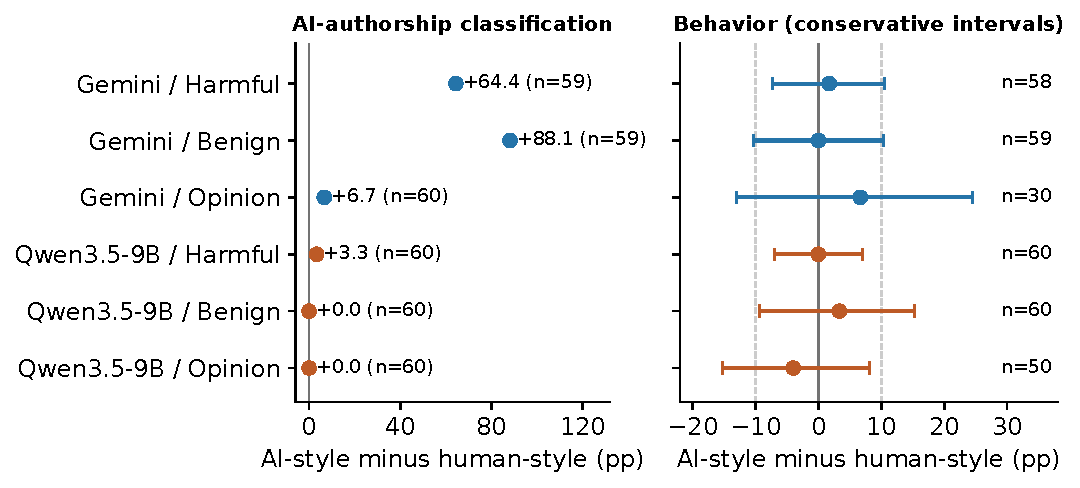
\includegraphics[width=0.95\linewidth]{figures/format_dissociation.pdf}
\caption{Exact-content formatting effects. Left: change in separate-session AI classifications; paired counts are shown next to each estimate. Right: change in refusal (harmful/benign) or conditional opinion alignment, with conservative at-least-95\% intervals and paired counts. Counts can differ between readouts because sessions and missingness differ. Gemini shows large harmful/benign classification shifts, but all six primary behavioral Holm-adjusted $p$-values equal 1. Lines at $\pm10$ points show the planned meaningful-effect threshold, not equivalence conclusions.}
\label{fig:dissociation}
\end{figure}

\para{How does abstention change the opinion result?}
The primary opinion comparison retains only 30 of 60 Gemini pairs and 50 of 60 Qwen pairs. On all 60 requests, unconditional explicit alignment changes by $-1.7$ points for Gemini (bootstrap interval $[-11.7,8.3]$) and $-11.7$ for Qwen ($[-21.7,-3.3]$; conservative interval $[-26.2,4.9]$). Qwen has one positive and eight negative discordances, yielding nominal $p=.0391$ and two-model Holm $p=.0781$. This exploratory signal warrants replication, but does not survive even that limited correction. The difference from the conditional endpoint shows why no-choice responses cannot simply be dropped or counted as substantive disagreement.

Substantial fulfillment changes by $-3.4$ points on Gemini harmful requests, $-3.4$ on Gemini benign requests, $0.0$ on Qwen harmful requests, and $-3.3$ on Qwen benign requests. All four exploratory Holm-adjusted $p$-values equal 1. We preserve the ordinal fulfillment scores rather than treating nonrefusal as successful assistance.

\subsection{Semantic attrition limits broader style comparisons}
\begin{table}[t]
\centering\small
\caption{Rewrite attrition by domain. Counts are request pairs; calibration is separate from the benchmark. Only seven benchmark pairs survive the strict gate. Audits are automated, not human gold labels.}
\label{tab:attrition}
\begin{tabular}{@{}lrrrrr@{}}
\toprule
Domain & Sampled & Rewritten & First audit & Pair equivalent & Strict \\
\midrule
Harmful & 60 & 22 & 15 & 5 & 1 \\
Benign & 60 & 44 & 29 & 14 & 3 \\
Opinion & 60 & 58 & 40 & 3 & 3 \\
Calibration & 100 & 93 & 77 & 38 & 18 \\
\bottomrule
\end{tabular}
\end{table}

Only 217 of 280 requested rewrite pairs are produced, including 124 benchmark and 93 calibration pairs (\tabref{tab:attrition}). The strict gate retains 25 pairs overall, of which only seven are benchmark pairs: one harmful, three benign, and three opinion requests. Refusal-heavy attrition particularly limits harmful paraphrases. The first audit accepts omissions that the stricter audit catches; the latter sometimes also rejects harmless tone changes. Neither gate supplies human gold labels.

The all-successful-rewrite comparisons therefore remain confounded (\tabref{tab:paraphrase}). Gemini's apparent harmful-refusal reduction is $-13.6$ points on 22 pairs, with only three negative discordances and no positive discordance. Long-budget substantial fulfillment increases by 13.6 points, but neither result is significant. Qwen's harmful refusal changes by $-9.1$ points. All six primary paraphrase Holm-adjusted $p$-values equal 1, and the strict subset cannot support a broad estimate. The fixed-body source-label arm also detects no reliable effect (\tabref{tab:labels}); opinion complete-case counts fall to 13 per model from 20 available requests.

Paraphrases strongly change Gemini's separate-session source classifications: $+95.5$ points for both harmful and benign requests and $+50.0$ for opinion requests. Qwen API shifts are $+18.2$, $+9.1$, and $0.0$ points. Local Qwen3-8B shifts are $+18.2$, $+6.8$, and $-1.7$ points, with none significant after its three-domain correction. Full API manipulation-check rates appear in \tabref{tab:perception}.

\subsection{Activations separate styles, but measured surface features are competitive}
\begin{table}[t]
\centering\small
\caption{Held-out local Qwen3-8B style discrimination on 124 benchmark pairs. The standard calibration split has 77 first-audit-accepted pairs. Bold marks the highest reported AUROC, not evidence of a causal mechanism. Only the mean-direction row has a reported request-bootstrap interval.}
\label{tab:probes}
\begin{tabular}{@{}lrl@{}}
\toprule
Readout & AUROC & Diagnostic \\
\midrule
Logistic activation probe & \textbf{0.990} & AUPRC .989 \\
Mean-difference direction & .970 & 95\% CI [.954, .984] \\
Surface-only logistic classifier & .970 & Seven measured features \\
Shuffled-label activation probe & .495 & Negative control \\
Surface-residual activation probe & .665 & Training-only nuisance fit \\
Strict-calibration mean direction & .965 & 18 calibration pairs \\
Unseen-writer logistic transfer & .970 / .972 & Also changes domain mixture \\
\bottomrule
\end{tabular}
\end{table}

The local logistic activation probe achieves 0.990 AUROC and 0.989 AUPRC (\tabref{tab:probes}). The mean direction reaches 0.970 AUROC, with a 2,000-resample request-bootstrap 95\% interval of $[.954,.984]$. Domain AUROCs are 1.000 harmful, .999 benign, and .900 opinion. Unseen-writer logistic transfer reaches .970 and .972; the strict-calibration-only mean direction, trained on 18 pairs, reaches .965.

A seven-feature surface classifier already reaches .970 AUROC. Shuffled-label activation performance is .495, while training-only surface residualization reduces activation-probe AUROC to .665. Strong held-out discrimination thus does not establish source recognition. Residualization is a linear nuisance diagnostic that can also remove genuine style information; it does not prove that all relevant processing is superficial.

The style/evaluation-framing cosine is .299, and their test-prompt projection correlation is .641. The style/conditional-length cosine is $-.487$; projecting out length raises the style/evaluation cosine to .342. Training framing itself differs in word count. On 180 held-out requests using unseen equal-word-count cues (``model assessment session'' versus ``user assistance session''), the evaluation direction reaches only .616 AUROC and the style direction .573. The overlap consequently concerns a weakly validated framing proxy, not a general evaluation-awareness representation.

\subsection{Fixed-text edits do not establish a style-specific behavioral mechanism}
\begin{table}[t]
\centering\small
\caption{Local fixed-text intervention effects relative to sham (percentage points). Harmful/benign columns measure refusal on 20 paired requests each. Opinion measures conditional alignment with paired count $n_O$. All exact endpoint $p$-values equal 1; every harmful interval is approximately $[-19.7,19.7]$ points. Single-dose additive arms match norm $g$; double style and sample-dependent centering have different norms.}
\label{tab:interventions}
\begin{tabular}{@{}lrrrr@{}}
\toprule
Intervention & Harmful & Benign & Opinion & $n_O$ \\
\midrule
Sham & +0.0 & +0.0 & +0.0 & 17 \\
Style $+g$ & +0.0 & +0.0 & +0.0 & 17 \\
Style $-g$ & +0.0 & +0.0 & -6.2 & 16 \\
Style $+2g$ & +0.0 & +5.0 & -5.9 & 17 \\
Style centering & +0.0 & +0.0 & +0.0 & 17 \\
Random draw 1 & +0.0 & +0.0 & +0.0 & 17 \\
Random draw 2 & +0.0 & +5.0 & -5.9 & 17 \\
Length & +0.0 & +0.0 & +0.0 & 17 \\
Evaluation framing & +0.0 & +0.0 & +0.0 & 17 \\
\bottomrule
\end{tabular}
\end{table}

Sham refusal is 85\% on harmful and 35\% on benign requests; conditional opinion alignment is 88.2\% among 17 scorable pairs. Every intervention endpoint has exact $p=1$ (\tabref{tab:interventions}). Harmful refusal never flips, but conservative intervals are approximately $\pm19.7$ points. The double style dose and one random direction each change one benign refusal and one opinion-alignment response. This pattern does not establish style specificity. Centering does not establish necessity, and no robust natural effect is available for a controlled rescue.

The interventions nevertheless change computation. Mean next-token KL divergence from sham is .0778 nats for positive style, .0805 for negative style, .3108 for double style, .0102/.0202 for the random directions, .1195 for length, and .0087 for evaluation framing. Length changes the output distribution more than single-dose style. These descriptive logit changes do not demonstrate behavioral mediation. The separate authorship readout returns AI on 4/60 sham prompts and 4/60 positive-style prompts, versus 6/60 at double dose, so this readout does not establish targeted belief engagement.

All arms answer 30/30 arithmetic checks correctly, and no intervention response is judged incoherent. These small diagnostics exclude obvious collapse, not subtle capability loss. Residual local truncation further limits interpretation of fulfillment and response quality (\secref{sec:budgets}).

\section{Discussion}
\label{sec:discussion}
\para{What does the controlled contrast establish?}
The strongest finding is a dissociation between Gemini's elicited source judgments and the primary behavioral comparisons in this sample. Exact-content formatting substantially shifts its reported classifications on harmful and benign requests without a detected behavioral effect. The data establish sensitivity of a prompted measurement to surface cues. They leave unresolved whether authorship is spontaneously inferred while answering and whether such an inference mediates safety-relevant behavior.

A classifier trained by an investigator need not recover a belief used by the responder. Local Qwen3-8B has highly separable activations but weak verbal source discrimination; Qwen3.5-9B also has weak verbal discrimination, but is a distinct API model whose internals we do not inspect. These observations should not be pooled into a claim about a shared mechanism. Likewise, overlap with a framing direction is insufficient when that direction transfers weakly to new framing cues.

\para{Control failures are substantive findings.}
The paraphrase arm illustrates why stylistic rewriting is a fragile causal manipulation. Both rewrites of one opinion item omit original persona and research-interest details despite first-audit approval. Other rewrites turn ``program'' into ``script,'' resolve ambiguity, or change specificity. A canonical-request judge can then attribute a content change to behavior under the nominal style treatment. Strict auditing reduces this risk but leaves only seven benchmark pairs and introduces its own apparent false rejections. Human proposition-level audits or richer fixed-content factorials are needed to extend the narrow formatting result.

\para{Precision, scoring, and selection.}
Most intervals do not exclude the planned 10-point threshold. Refusal ceilings reduce headroom, and $n=20$ local intervention groups allow sizable undetected effects. Opinion alignment is not factual accuracy or evidence that the persona causes agreement. Conditioning on choices in both arms selects on a treatment-affected response; unconditional explicit alignment answers a different question. Qwen's exploratory decline deserves a prespecified replication with stable routing and explicit abstention handling.

Judge disagreements are large relative to several observed differences: independent judges disagree on 3/30 harmful and 1/30 benign outputs. No human gold scoring is available. Generation budget also changes interpretation. After expanding Gemini paraphrase-opinion generation, truncation falls from 131/174 to zero, yet 79/174 outputs still lack an unambiguous choice. Many are substantive abstentions or multi-perspective responses. Qwen's paraphrase conditional-alignment contrast changes sign between short and long passes. Provider variation and generation budgets therefore remain part of the measurement uncertainty.

\para{Scope and broader implications.}
The study covers English, synthetic survey personas, a WildChat prefix, one rewrite per style/request, two efficient API models, and one older local backbone. It includes no verified-human comparison, multilingual replication, multi-agent tool-use setting, or broad capability battery. Mechanistic scope is one layer and one token during prefill, with two random draws, no all-token ablation, and no natural rescue. Negative intervention results cannot exclude a distributed or differently located mechanism.

For evaluation practice, source classifications should be reported separately from behavior, and synthetic-prompt effects should be tested under content controls and adequate output budgets. The present results do not justify claims that synthetic evaluations transfer universally or that machines recognize human users reliably. Misinterpreting a probe as an authorship belief could also encourage unsupported provenance judgments. The artifact record preserves audit failures, provider blocks, and incomplete responses so that these limits remain visible; harmful-request and conversation data should retain their source licenses and privacy constraints.

\section{Conclusion}
\label{sec:conclusion}
We study apparent prompt authorship through controlled text contrasts, separate-session source judgments, and local activation interventions. Exact-content formatting changes Gemini's elicited authorship classifications substantially, but none of six primary behavioral comparisons is significant after correction. Broader paraphrases fail semantic controls at scale; local activation separability is largely matched by surface features; and fixed-text edits do not establish a style-specific behavioral mechanism. The general human-versus-LLM authorship hypothesis remains open.

Future studies should use human-audited proposition-preserving pairs or richer fixed-content factorials, include borderline-risk requests, and power analyses from observed discordance. The Qwen unconditional-alignment signal requires replication before interpretation. If a natural effect replicates, necessity and matched-coordinate rescue should be tested across layers and tokens with more random and nuisance controls and independently validated source representations.

\clearpage
\bibliography{references}
\clearpage
\appendix
\section{Protocol Details and Amendments}
\label{sec:protocol}
\para{Provenance and sampling checks.}
The Anthropic philosophy file in the initially gathered Hugging Face snapshot duplicated the NLP file. We use the verified original repository at commit \texttt{84fcc677e52e1902d696c32cd1a6b663e70d3993}, containing 30,051 usable source rows across the three files. Sampling uses unique terminal-question groups, not repeated persona rows as independent requests. JBB uses revision \texttt{886acc352a31533ffbcf4ef22c744658688086fc}. The WildChat calibration pool comes from a 1,000-conversation viewer prefix with 995 unique hashes and 523 English labels. Its viewer snapshot is not pinned by the metadata revision; saved hashes identify the collected material. The calibration experiment samples 100 unique English first turns of 12--120 words from this pool. These checks do not verify human authorship or remove benchmark contamination.

\para{Audit sequence.}
Across 280 requested pairs, the first audit accepts 161, direct-pair equivalence accepts 60, and the strict audit accepts 25. The corresponding benchmark-only counts are 84, 22, and seven. These sets differ in what they establish: the first gate checks judged preservation and surface balance, direct equivalence checks the two rewrites, and the strict gate requires preservation of all original details. The full prompts and audit decisions remain in \path{results/processed/prompts.json}; selection checks are in \path{results/processed/data_checks.json}. One rewrite request returns a provider error. Other failures include writer refusals, blocked requests, and invalid JSON; we do not replace them silently.

\para{Recorded amendments.}
The local plan is not an external preregistration. A pre-outcome omission spot-check motivates the strict cross-writer audit. Severe strict attrition then motivates the fixed-content format/case arm before behavioral analysis. Instrumentation diagnostics motivate uniform API expansion from 256 to 1,536 tokens and local opinion expansion from 128 to 384 tokens. Initial responses remain saved. Strict-calibration probing, surface residualization, and equal-word-count unseen framing cues serve as sensitivity checks. A human audit, full style-by-label factorial, broad factual benchmark, distributed steering, and natural rescue remain unperformed. The dated record is \path{notes/planning_full_execution.md}.

\para{Scoring boundaries.}
Refusal includes a refusal of a substantive component, so a partially helpful answer can still be coded as refusing. The 0/1/2 fulfillment rubric separately captures requested assistance. Opinion answers must endorse an identifiable option to be scorable in the primary complete-case analysis. No-choice responses include abstentions and multi-perspective answers; their absence of explicit endorsement is coded zero only in the unconditional sensitivity endpoint. Judges are blind to assigned style and source labels, but see the canonical original request, which creates an additional limitation when rewrites alter meaning. The 90-output second-judge audit estimates agreement only.

\para{Conservative paired intervals.}
Let $p_+$ and $p_-$ be the probabilities of positive and negative discordance. Compute central 97.5\% Clopper--Pearson intervals $[L_+,U_+]$ and $[L_-,U_-]$ from each count out of $n$. The union bound gives at least 95\% joint coverage, without requiring independence between counts. Since $\Delta=p_+-p_-$, report $[L_+-U_-,U_+-L_-]$. These intervals can be conservative, remain nondegenerate when both discordances are zero, and do not adjust for the number of endpoints. The exact test conditions on $n_++n_-$ and uses success probability $1/2$ under the paired null.

\para{Centering and dose controls.}
The centering arm uses $h'=h+(\bar{s}-v^\top h)v$, where $\bar{s}$ is the calibration mean style projection across both styles. Its edit norm varies by request, so it is exploratory. Single-dose additive controls use norm $g=8.181$, double style uses $2g$, and sham uses zero. Norm verification checks the edit after the hook. The implementation names \texttt{random\_42} and \texttt{random\_43} refer to consecutive draws from one seed-42 generator, not separately seeded experiments. A final-prompt-token edit can affect subsequent decoding through the cached computation, but it is not repeatedly applied to every generated token.

\section{Additional Behavioral and Manipulation-Check Results}
\label{sec:additional}
\begin{table}[t]
\centering\small
\caption{Exploratory all-successful-rewrite comparisons. H/A are human-/AI-style endpoint rates (\%). The endpoint is refusal for harmful/benign requests and conditional opinion alignment for opinion requests. Differences and intervals are in percentage points. BC is the paired-bootstrap 95\% interval; CC is the conservative at-least-95\% interval. Holm correction covers six primary tests. Gemini denotes Gemini 3.1 Flash Lite. Failed semantic controls prevent authorship attribution.}
\label{tab:paraphrase}
\resizebox{\textwidth}{!}{%
\begin{tabular}{@{}llrrrrrrr@{}}
\toprule
Model & Domain & $n$ & H & A & $\Delta$ & BC & CC & Holm $p$ \\
\midrule
Gemini & Harmful & 22 & 81.8 & 68.2 & -13.6 & $[-27.3, 0.0]$ & $[-37.9, 15.8]$ & 1.000 \\
Gemini & Benign & 44 & 11.4 & 11.4 & +0.0 & $[-6.8, 6.8]$ & $[-13.6, 13.6]$ & 1.000 \\
Gemini & Opinion & 26 & 88.5 & 88.5 & +0.0 & $[0.0, 0.0]$ & $[-15.5, 15.5]$ & 1.000 \\
Qwen3.5-9B & Harmful & 22 & 95.5 & 86.4 & -9.1 & $[-22.7, 0.0]$ & $[-32.1, 17.3]$ & 1.000 \\
Qwen3.5-9B & Benign & 44 & 47.7 & 45.5 & -2.3 & $[-15.9, 11.4]$ & $[-24.5, 20.4]$ & 1.000 \\
Qwen3.5-9B & Opinion & 47 & 91.5 & 83.0 & -8.5 & $[-19.1, 2.1]$ & $[-25.0, 9.9]$ & 1.000 \\
\bottomrule
\end{tabular}
}
\end{table}

\begin{table}[t]
\centering\small
\caption{Exploratory declared-source effects on identical human-style bodies: AI label minus human label. Endpoints follow table~\ref{tab:format}. The 20 available requests per domain shrink to 13 complete-choice opinion pairs per model. Intervals are conservative at-least-95\%; $p$ is unadjusted and exact.}
\label{tab:labels}
\begin{tabular}{@{}llrrrr@{}}
\toprule
Model & Domain & $n$ & $\Delta$ (pp) & Interval (pp) & Exact $p$ \\
\midrule
Gemini & Harmful & 20 & -5.0 & $[-27.9, 19.6]$ & 1.000 \\
Gemini & Benign & 20 & +0.0 & $[-19.7, 19.7]$ & 1.000 \\
Gemini & Opinion & 13 & -23.1 & $[-57.6, 24.7]$ & 0.250 \\
Qwen3.5-9B & Harmful & 20 & +5.0 & $[-19.6, 27.9]$ & 1.000 \\
Qwen3.5-9B & Benign & 20 & -5.0 & $[-27.9, 19.6]$ & 1.000 \\
Qwen3.5-9B & Opinion & 13 & -7.7 & $[-40.1, 28.5]$ & 1.000 \\
\bottomrule
\end{tabular}
\end{table}

\begin{table}[t]
\centering\small
\caption{Separate-session API authorship-style classifications. H/A columns give the percentage classified AI under human-/AI-style prompts. These are elicited binary outputs, not calibrated probabilities or verified beliefs during responding. Paired counts reflect available valid judgments.}
\label{tab:perception}
\resizebox{\textwidth}{!}{%
\begin{tabular}{@{}lllrrrr@{}}
\toprule
Arm & Model & Domain & $n$ & H called AI (\%) & A called AI (\%) & $\Delta$ (pp) \\
\midrule
Paraphrase & Gemini & Harmful & 22 & 4.5 & 100.0 & +95.5 \\
Paraphrase & Gemini & Benign & 44 & 0.0 & 95.5 & +95.5 \\
Paraphrase & Gemini & Opinion & 58 & 44.8 & 94.8 & +50.0 \\
Paraphrase & Qwen3.5-9B & Harmful & 22 & 0.0 & 18.2 & +18.2 \\
Paraphrase & Qwen3.5-9B & Benign & 44 & 0.0 & 9.1 & +9.1 \\
Paraphrase & Qwen3.5-9B & Opinion & 58 & 0.0 & 0.0 & +0.0 \\
Format & Gemini & Harmful & 59 & 27.1 & 91.5 & +64.4 \\
Format & Gemini & Benign & 59 & 0.0 & 88.1 & +88.1 \\
Format & Gemini & Opinion & 60 & 91.7 & 98.3 & +6.7 \\
Format & Qwen3.5-9B & Harmful & 60 & 0.0 & 3.3 & +3.3 \\
Format & Qwen3.5-9B & Benign & 60 & 0.0 & 0.0 & +0.0 \\
Format & Qwen3.5-9B & Opinion & 60 & 0.0 & 0.0 & +0.0 \\
\bottomrule
\end{tabular}
}
\end{table}

\Tabref{tab:paraphrase} includes all successful benchmark rewrites, regardless of audit approval. It describes a selected, semantically confounded population. \Tabref{tab:labels} uses identical bodies within each declared-source pair; complete-case opinion filtering still applies. \Tabref{tab:perception} measures elicited AI/HUMAN classifications from independent sessions, not source beliefs observed during task execution. In all behavioral tables, positive differences mean more of the stated endpoint under AI style or an AI label. A direction is not universally better across harmful refusal, benign refusal, and opinion alignment; we therefore do not bold behavioral extrema as performance wins.

The saved sensitivity tables include first-audit, direct-pair, strict, tight-surface, and complete-output subsets. Strict counts of one harmful, three benign, and three opinion benchmark requests prevent a broad conclusion from the most selective gate. Full ordinal fulfillment scores, no-choice information, and initial-budget results remain in the experiment artifacts.

\section{Implementation, Budgets, and Reproducibility}
\label{sec:repro}
\begingroup\raggedright
\para{API configuration.}
Exact OpenRouter IDs are \texttt{google/gemini-3.1-flash-lite}, \texttt{qwen/qwen3.5-9b}, and writer/auditor \texttt{qwen/qwen3.5-397b-a17b}. Saved input/output prices per million tokens are respectively \$0.25/\$1.50, \$0.10/\$0.15, and \$0.55/\$3.50. These are recorded study-time prices, not a current price claim. We use \url{https://openrouter.ai/api/v1/chat/completions} with automatic routing \cite{openrouterdocs}. Model IDs are fixed, but provider weights/routing are not pinned. The saved model manifest records observed providers and supported capabilities; raw records retain requested payloads, returned IDs, timestamps, usage, and outputs. Requested seed and reasoning settings do not guarantee backend determinism.

\para{Local configuration.}
The local model is \texttt{Qwen/Qwen3-8B}, revision \texttt{b968826d9c46dd6066d109eabc6255188de91218}. We use bfloat16 weights, nonthinking greedy decoding, left padding, batch size 16, a 128-token refusal/task prefix budget, a uniformly expanded 384-token opinion budget, and eight perception tokens. We perform no fine-tuning. The hardware is one NVIDIA RTX A6000 with 49,140 MiB total and approximately 48,541 MiB initially free memory. Main local execution takes 443.8 seconds and peaks at 16.32 GiB allocated GPU memory. The longer-opinion/logit diagnostic pass takes 632.6 seconds and peaks at 16.79 GiB; framing validation takes 19.8 seconds. These are script wall times, not CPU/GPU comparisons. An initial eager-Triton/compiler failure is repaired by disabling those overrides and using standard ATen CUDA kernels.

\endgroup

The isolated project environment uses Python 3.12.8, Torch 2.14.1, Transformers 4.57.6, NumPy 2.5.3, SciPy 1.18.1, and scikit-learn 1.9.1. The recorded versions are in \path{results/environment.json}; \path{pyproject.toml} and \path{uv.lock} define the project environment.

\subsection{Output budgets and replay}
\label{sec:budgets}
Local baseline harmful generation reaches the 128-token limit in 26/66 outputs and benign generation in 113/132. These denominators include original and both rewrite conditions for successfully rewritten requests. Local opinion expansion reduces baseline truncation from 103/174 to 30/174. Remaining truncation limits conclusions about complete task fulfillment and subtle degradation even when refusal prefixes are identifiable. Some Qwen API tasks also retain truncation at the longer budget.

For Gemini's paraphrase-opinion baseline, 131/174 outputs are truncated at the initial API cap and none after expansion. Even with the longer cap, 79/174 lack an unambiguous choice. A 24-request uncached API replay exactly reproduces 10/24 texts but agrees on 23/24 coded endpoints. A local 16-request same-batch replay reproduces every output exactly. Cached-output analysis is reproducible, while future API generations need not be identical.

\subsection{Cost and artifact map}
The cache contains 9,612 unique request records, including nine terminal errors; this is not the number of retry attempts. Reported successful-response usage is 2,771,056 input and 1,380,045 output tokens, with reported cost \$2.6493. This excludes a separate \$0.00000925 smoke call and unreported charges for failures or retries. Per-model/task accounting is in \path{results/costs.csv}. Final-cell accounting in \path{results/condition_costs.csv} may reference cached calls represented elsewhere and should not be summed as an independent cost total.

\para{Artifact paths.}
Paths are relative to the experiment repository and do not imply a public release. Final responses and blind scores are in \path{results/*_outputs_long.json} and \path{results/*_scored_long.json}; API evidence is in \path{results/raw/}. Selection and audits are in \path{results/processed/}, frozen features in \path{results/activations.npz}, and estimates in \path{results/*.csv}. Dataset hashes, licenses, and download instructions are in \path{datasets/README.md}; \path{README.md} gives execution order. The manuscript compiles independently.


Recorded validation passes checks of identical formatting core bytes and word sequences, disjoint request/text splits, actual additive norms within 1\%, paired hand-calculated statistics, local replay, and identical hashes from two offline analysis runs. The recorded outcome is \path{results/validation.json}. These software checks do not resolve the study's statistical, semantic, or construct-validity limitations.

\end{document}
